\documentclass[sigconf,anonymous]{acmart}
%% Converted from IEEEtran to the ACM "acmart" sigconf template.
%% "anonymous" hides the author block and \shortauthors for KDD's
%% double-blind review. No "review" option => no line numbers.
%% For the camera-ready, swap in [sigconf,screen] and fill in
%% \acmConference/\copyrightyear/\acmDOI/\acmISBN.

%% acmart is built on the amsart class, which already natively provides
%% amsmath, amssymb, amsthm, \newtheorem/\theoremstyle, and the "proof"
%% environment. Reloading amsthm or amssymb here collides with those
%% (amsthm breaks "proof"; amssymb redefines \Bbbk) -- do not add them.
\usepackage{amsmath}
\usepackage{algorithm}
\usepackage{algorithmic}
%% acmart already loads xcolor (with the "prologue" option) and
%% booktabs/graphicx/hyperref/microtype, so we only add what is
%% missing: colortbl gives \rowcolor without re-loading xcolor
%% (re-loading it with different options would raise an option clash).
\usepackage{colortbl}
\usepackage{enumitem}
\usepackage[most]{tcolorbox}

% ── theorem environments (plain amsthm; no colour) ──────────────────
\theoremstyle{plain}
\newtheorem{theorem}{Theorem}
\newtheorem{lemma}{Lemma}
\newtheorem{proposition}{Proposition}
\newtheorem{corollary}{Corollary}
\theoremstyle{definition}
\newtheorem{definition}{Definition}
\newtheorem{assumption}{Assumption}
\theoremstyle{remark}
\newtheorem{remark}{Remark}

% ── colours: ONLY for the Core-idea callout and tables ──────────────
\definecolor{navyblue}{HTML}{1F4E79}
\definecolor{insln}{HTML}{B8860B}
\definecolor{insbg}{HTML}{FBF4E2}
\definecolor{headrow}{HTML}{1F4E79}
\definecolor{oursrow}{HTML}{E8F8E8}

% Core-idea callout box (the only coloured text box in the paper)
\newtcolorbox{insightbox}{enhanced jigsaw, breakable, boxrule=0pt, boxsep=0pt,
  colback=insbg, sharp corners, left=8pt, right=6pt, top=4pt, bottom=4pt,
  borderline west={2.4pt}{0pt}{insln}, before skip=6pt, after skip=6pt}

\hypersetup{colorlinks=true, linkcolor=navyblue, citecolor=navyblue,
  urlcolor=navyblue, breaklinks=true}

\AtBeginDocument{\providecommand\BibTeX{{Bib\TeX}}}

\begin{document}

\title[Trust-Gated Capability Control]{Trust-Gated Capability Control: An Operational Framework for Breaking the
Trust--Vulnerability Paradox in Multi-Agent LLM Systems}

%% Target venue: KDD '27 (submission).  Sets the running-header and
%% ACM Reference Format venue string.  Copyright/DOI/ISBN remain as
%% acmart placeholders and will be replaced automatically by the ACM
%% at camera-ready time.
\acmConference[KDD '27]{The 33rd ACM SIGKDD Conference on Knowledge
  Discovery and Data Mining}{August 2027}{San Jose, CA, USA}
\acmYear{2027}
\copyrightyear{2027}

\author{Md Mehedi Hasan Bhuiyan Nipu}
\affiliation{%
  \institution{North South University}
  \city{Dhaka}
  \country{Bangladesh}}

\author{Mohammad Sakib Mahmood}
\affiliation{%
  \institution{Missouri State University}
  \city{Springfield}
  \state{MO}
  \country{USA}}

\author{Md. Jakir Hossen}
\affiliation{%
  \institution{Multimedia University}
  \city{Melaka}
  \country{Malaysia}}

\author{M. F. Mridha}
\affiliation{%
  \institution{American International University--Bangladesh}
  \city{Dhaka}
  \country{Bangladesh}}

\renewcommand{\shortauthors}{Nipu et al.}

\begin{abstract}
Layered trust models for multi-agent large language model (LLM) systems remain largely
conceptual: they describe which dimensions of trust matter but do not specify how trust
at different layers combines, how layer importance adapts at runtime, or how trust should
govern what an agent is permitted to do. This gap is consequential because increasing
inter-agent trust raises task success while simultaneously enlarging exposure to
adversarial exploitation, a tension formalized as the Trust-Vulnerability Paradox (TVP).
We make a five-layer trust stack operational. We first introduce a cross-layer synergy
operator that encodes layer dependencies through a lower-triangular coupling matrix, and
a generalized power-mean composite trust that admits a closed-form conservative fixed
point and provable bounds. We then prove that failure-grounded multiplicative-weights
estimation of layer importance converges geometrically and is no-regret. Building on
these, we introduce Trust-Gated Capability Control (TGCC): a runtime mechanism that
issues short-lived, revocable capability grants conditioned on both composite trust and
per-prerequisite-layer thresholds. We prove that TGCC breaks the paradox, that its
revocation latency is logarithmic, and that the false-positive rate for honest agents
decays exponentially with interaction length. A deployment-time threshold-calibration
procedure with a sample-complexity guarantee connects the theory to practice. Five
experiments validate the framework: a real-LLM epistemic calibration probe shows the
synergy operator reduces over-exposure by a factor of $4.2$ against a no-synergy
baseline; a multi-agent debate study confirms complete sleeper revocation across team
sizes; an ablation identifies the practical operating region; a code-generation pipeline
blocks $95\%$ of harmful commits; and a scalability study confirms constant per-agent
overhead through fifty agents, empirically validating the quadratic complexity bound.
An extended robustness study of eleven further experiments (Appendix~\ref{app:robustness_ext})
addresses statistical significance, colluding adversaries, indirect prompt injection,
per-layer attribution, long-horizon drift, parameter sensitivity, revocation-then-recovery,
Byzantine chains, auditability, calibration robustness, and adaptive attackers.
\end{abstract}

%% Best-effort CCS placeholders -- regenerate the numeric concept IDs
%% at https://dl.acm.org/ccs.cfm before camera-ready submission.
\begin{CCSXML}
<ccs2012>
 <concept>
  <concept_id>00000000.0000000.0000000</concept_id>
  <concept_desc>Security and privacy~Systems security</concept_desc>
  <concept_significance>500</concept_significance>
 </concept>
 <concept>
  <concept_id>00000000.00000000.00000000</concept_id>
  <concept_desc>Security and privacy~Access control</concept_desc>
  <concept_significance>400</concept_significance>
 </concept>
 <concept>
  <concept_id>00000000.00000000.00000000</concept_id>
  <concept_desc>Computing methodologies~Multi-agent systems</concept_desc>
  <concept_significance>400</concept_significance>
 </concept>
 <concept>
  <concept_id>00000000.00000000.00000000</concept_id>
  <concept_desc>Computing methodologies~Online learning settings</concept_desc>
  <concept_significance>100</concept_significance>
 </concept>
</ccs2012>
\end{CCSXML}

\ccsdesc[500]{Security and privacy~Systems security}
\ccsdesc[400]{Security and privacy~Access control}
\ccsdesc[400]{Computing methodologies~Multi-agent systems}
\ccsdesc[100]{Computing methodologies~Online learning settings}

\keywords{Multi-agent systems, large language models, trust management, zero-trust
architecture, capability-based security, agent safety, alignment, calibration, online
learning, power-mean aggregation, threshold calibration, adversarial robustness}

\maketitle

% ══════════════════════════════════════════════════════════════════════
\section{Introduction}
\label{sec:intro}
% ══════════════════════════════════════════════════════════════════════
Large language model (LLM) agents are no longer deployed only as solitary assistants.
They are increasingly composed into \emph{collectives} that plan, negotiate, delegate,
and act through shared tools, memories, and message
channels~\cite{wang2024survey,guo2024llmmultiagent,tran2025multiagent,hong2308metagpt}.
Such collectives already drive software engineering pipelines, scientific-discovery
workflows, clinical-decision support, and autonomous web agents. As autonomy and
interconnection grow, the behaviour of any one agent becomes consequential for the
entire system: an output that is consumed downstream without scrutiny can silently
propagate errors, and a single subverted participant can compromise a whole workflow.
Collaboration, in other words, converts \emph{trust} between agents from a background
assumption into a first-class operational variable that must be measured, reasoned about,
and acted upon at runtime.

Recent empirical work has made this concern precise. Structured attacks that exploit
inter-agent trust raise harmful-response rates well above single-agent
baselines~\cite{qi2025amplified}, and a growing body of evidence shows that trust and
vulnerability are coupled rather than independent. Specifically, raising the degree to
which agents accept one another's claims improves task success but simultaneously
enlarges the attack surface, a phenomenon recently formalized as the
\emph{Trust-Vulnerability Paradox} (TVP)~\cite{qi2025trust}. The lesson echoes the
zero-trust movement in systems security: trust should never be implicit, should be
continuously re-verified, and should be coupled to least-privilege
authorization~\cite{zerotrust2025,trism2026,nist800207}. Yet translating that principle
into a concrete, runtime decision rule for LLM collectives remains an open problem.

\textbf{The conceptual--operational gap.}
A natural and increasingly popular response is to model trustworthiness as a
\emph{layered stack}, decomposing it into dimensions such as epistemic reliability,
behavioural alignment, role adherence, social accountability, and institutional
governance. Layered models are attractive because they separate concerns and map onto
distinct measurement instruments. However, the existing accounts are almost entirely
\emph{descriptive}. They tell us \emph{which} dimensions matter, but they leave three
operational questions unanswered. First, \emph{composition}: given that the layers are
not independent---epistemic failure undermines every higher layer---how should the
layer-wise trust values be combined into a single, actionable score? Second,
\emph{weighting}: how is the relative importance of each layer set, and can that
importance adapt to whichever layer is currently failing? Third, \emph{actuation}: once a
composite trust score exists, how should it govern what an agent is permitted to do, and
how quickly can permissions be withdrawn? Without principled answers to all three, a
layered model is a taxonomy, not a controller, and cannot be deployed in a
safety-critical setting.

\textbf{A motivating scenario.}
Consider a clinical pipeline ending in a \emph{scribe} agent that holds a high-risk
\emph{write-to-EHR} capability. Suppose an upstream \emph{reasoner} is compromised so
that it returns plausible-sounding but incorrect inferences with high stated confidence,
while remaining cooperative and articulate in tone. A controller that authorizes the
write based on apparent helpfulness sees nothing wrong---fluent, well-formatted, and
professional---so incorrect conclusions are committed to patient records. This is the TVP
in microcosm: behavioural agreeableness masks a collapse of epistemic reliability, and a
trust signal that conflates the two is exploited. The defence we seek must detect that the
\emph{prerequisite} layer has failed even though the \emph{visible} layer appears
healthy, and withdraw the capability before harm is done. We return to this scenario in
Appendix~\ref{app:casestudy} once TGCC is fully defined.

\textbf{Why existing solutions fall short.}
Scalar reputation systems cannot represent a layer-specific failure hidden behind
cooperative behaviour~\cite{ramchurn2004trust,josang2002beta}; zero-trust policies
advocate per-call revocation but give no decision rule for \emph{when} to revoke on
multi-dimensional evidence~\cite{zerotrust2025,nist800207}; the defences proposed
alongside the TVP operate \emph{around} the trust signal rather than reshaping how it is
computed~\cite{qi2025trust}; and training-time alignment~\cite{christiano2017deep,
ouyang2022training,bai2022constitutional} shapes dispositions but provides no runtime
mechanism against an agent that turns adversarial after deployment. None of these lines
provides a compositional, runtime-operational trust framework with provable guarantees.

\textbf{Our approach.}
We treat the layered trust stack as a \emph{dynamical object} made operational through
four connected components: a \emph{cross-layer synergy operator} that propagates a
prerequisite-layer deficit upward and discounts every layer that depends on it; a
power-mean \emph{composite} that aggregates the effective per-layer trusts into a single
score dominated by the weakest verified layer; a failure-grounded
\emph{adaptive-weighting} rule that re-routes the composite's sensitivity toward whichever
layer is currently most responsible for harm; and \emph{Trust-Gated Capability Control}
(TGCC), which turns the composite into short-lived, revocable capability grants so that
authorization tracks the weakest verified layer rather than the easily inflated
behavioural layer. We prove that this construction breaks the TVP, bounds the time to
contain a compromise, and keeps false positives for honest agents exponentially rare.

\textbf{Contributions.}
\begin{itemize}[leftmargin=1.2em,topsep=2pt,itemsep=2pt]
\item We formalize the multi-agent trust-gating problem and the Trust-Vulnerability
  Paradox as a precise property of authorization policies
  (Section~\ref{sec:model_system}).
\item We introduce a cross-layer synergy operator and a generalized power-mean composite
  trust, and establish a closed-form conservative fixed point, tight bounds, a
  weakest-link limit, monotonicity, and sensitivity properties (Section~\ref{sec:model}).
\item We ground per-layer importance weights in observed failures and prove that the
  resulting estimator is no-regret and converges geometrically
  (Section~\ref{sec:weights}).
\item We present the TGCC algorithm and prove that it has constant per-step overhead,
  that it breaks the paradox, that its revocation latency is logarithmic, and that the
  false-positive rate decays exponentially (Section~\ref{sec:tgcc}).
\item We give a deployment-time threshold-calibration procedure with correctness and
  sample-complexity guarantees (Section~\ref{sec:calibration}), and additional
  adversarial-robustness results (Section~\ref{sec:robustness}).
\item We validate the framework with five experiments on real LLMs and simulation
  (Section~\ref{sec:experiments}), and provide a step-by-step deployment protocol
  (Section~\ref{sec:discussion}).
\item We complement the main study with a compact summary (Section~\ref{sec:exp_ext})
  and eleven further experiments (Appendix~\ref{app:robustness_ext}) covering statistical
  significance, colluding adversaries, prompt injection, per-layer attribution,
  long-horizon drift, parameter sensitivity, recovery, Byzantine chains, audit trails,
  calibration robustness, and adaptive attackers.
\end{itemize}
Extended derivations, a taxonomy of adversaries, additional aggregation-operator
comparisons, and further experimental figures are collected in the appendix so that the
main text stays focused on the operational core.

% ══════════════════════════════════════════════════════════════════════
\section{Related Work}
\label{sec:related}
% ══════════════════════════════════════════════════════════════════════

\textbf{Multi-agent LLM systems.}
Systems such as AutoGen~\cite{wu2023autogen}, CAMEL~\cite{li2023camel},
MetaGPT~\cite{hong2308metagpt}, ChatDev~\cite{qian2023chatdev}, and
AgentVerse~\cite{chen2023agentverse} orchestrate role-specialized agents through
structured dialogue, while embodied agents~\cite{wang2023voyager,park2023generative}
extend the paradigm to open-ended environments;
surveys~\cite{wang2024survey,guo2024llmmultiagent,tran2025multiagent} document a common
architecture of roles, messages, and tools. These works focus on \emph{capability},
whereas we focus on \emph{control}: bounding what a collective is permitted to do as a
function of measured trust. Our framework is complementary, protocol-agnostic, and can
wrap any of these systems.

\textbf{Trust as a security variable.}
The closest motivation for our work is the formalization of the
TVP~\cite{qi2025trust}, which isolates three facets of inter-agent trust---strength,
scope, and revocability---and shows that increasing scalar trust monotonically increases
both over-exposure and authorization drift; its defences reduce exposure but operate
around the trust signal rather than reshaping how it is computed. Zero-trust treatments
for agentic AI~\cite{zerotrust2025,nist800207} and the TRiSM
perspective~\cite{trism2026} advocate verifiable identity and continuous verification but
stop short of a concrete multi-layer decision rule; we supply exactly the missing rule.

\textbf{Reputation and probabilistic trust.}
Trust and reputation have a long history in multi-agent
systems~\cite{ramchurn2004trust,sabater2005review}, including
EigenTrust~\cite{kamvar2003eigentrust}, the Beta reputation
system~\cite{josang2002beta}, and subjective logic~\cite{josang2016subjective}; LLM-era
revivals include DynaTrust~\cite{dynatrust2026}, AgentGuard~\cite{agentguard2025}, and
economic-game trust elicitation~\cite{econgames2026}. These methods track a
\emph{single} trust quantity and are therefore blind to the core TVP scenario, in which
an agent is behaviourally cooperative yet epistemically broken. We retain the
mathematically convenient Beta machinery and prove a conservative fixed point for it, but
lift trust from a scalar to a coupled \emph{vector}, which is what makes a hidden
prerequisite failure visible.

\textbf{Debate, deception, and collective failure.}
Multi-agent debate can improve factuality~\cite{du2023debate,liang2023encouraging}, but
the same channels also enable harm: structured jailbreaks injected into one debater
amplify harmful responses~\cite{qi2025amplified}, and social deception simulations show
agents readily form, exploit, and misjudge trust~\cite{traitors2025}. Sleeper-agent
behaviour~\cite{hubinger2024sleeper} shows models can behave benignly until a trigger
condition is met---exactly the threat profile our controller contains.

\textbf{Uncertainty and calibration.}
The epistemic layer rests on knowing when an agent is wrong. Neural networks are
frequently miscalibrated~\cite{guo2017calibration}, and predictive uncertainty can be
quantified via Bayesian approximations~\cite{gal2016dropout}, deep
ensembles~\cite{lakshminarayanan2017simple}, semantic
entropy~\cite{kuhn2023semantic}, and selective prediction~\cite{geifman2017selective};
related work propagates epistemic state across collaborating agents~\cite{epistemic2026}.
Our synergy operator converts such a passive calibration measurement into an active
control input that gates downstream capabilities.

\textbf{Prompt injection, tool use, and capability security.}
Indirect prompt-injection~\cite{greshake2023not} and jailbreaks~\cite{wei2023jailbroken}
subvert an agent through its inputs, while tool-use
frameworks~\cite{schick2023toolformer,yao2023react} expand the actions an agent can take;
TGCC gates those actions on composite trust rather than detecting every input exploit.
Governing a principal via unforgeable, least-privilege tokens dates to capability-based
operating systems~\cite{dennis1966programming} and the object-capability
model~\cite{miller2006robust}, and underlies zero-trust
architecture~\cite{nist800207}; our grant rule is precisely such a capability-issuance
policy, short-lived and revoked the moment trust degrades.

\textbf{Online learning, aggregation, and Byzantine fault tolerance.}
Our adaptive weighting is an instance of the multiplicative-weights / Hedge
family~\cite{freund1997decision,arora2012mw,cesabianchi2006prediction}, and our composite
trust is a weighted power mean~\cite{hardy1952inequalities} related to ordered weighted
averaging~\cite{yager1988ordered} (Appendix~\ref{app:operators} justifies this choice).
Byzantine fault tolerance~\cite{lamport1982byzantine,castro1999practical} gives
correctness guarantees for a bounded fraction of arbitrary faults but assumes a $3f+1$
replication factor impractical for LLM agents; formal
verification~\cite{katz2017reluplex,gehr2018ai2} and temporal
monitoring~\cite{koymans1990specifying} likewise do not scale to the interaction space of
LLM collectives, so we trade hard certificates for probabilistic bounds. Our Beta
estimator with a forgetting factor is, in effect, a bank of online change-point
detectors~\cite{page1954continuous,basseville1993detection}, one per layer.

\textbf{Alignment, human--AI trust, and governance.}
RLHF~\cite{christiano2017deep,ouyang2022training}, constitutional
methods~\cite{bai2022constitutional}, red-teaming~\cite{perez2022red}, and
governance-graph collusion control~\cite{instai2026} address specific trust layers; since
deployed agents face non-stationary environments~\cite{gama2014survey}, our forgetting
factor keeps trust responsive to drift, and human--automation
calibration~\cite{lee2004trust} motivates our conservative fixed point (an over-eager
controller erodes honest agents just as over-trust endangers a human operator). These
works populate individual layers of our stack; we contribute the operator that composes
them and the controller that acts on the composite. Table~\ref{tab:positioning} in
Appendix~\ref{app:taxonomy} positions our approach against the most comparable lines of
work.

% ══════════════════════════════════════════════════════════════════════
\section{System Model and Problem Formulation}
\label{sec:model_system}
% ══════════════════════════════════════════════════════════════════════

\subsection{Multi-Agent LLM System}
A multi-agent LLM system is a tuple $\mathcal{S}=(\mathbb{A},\mathcal{C},\mathcal{P},\mathcal{K})$:
$\mathbb{A}=\{\mathcal{A}_1,\dots,\mathcal{A}_N\}$ is a finite set of agents, each backed by
an LLM; $\mathcal{C}$ is a finite set of \emph{capabilities} such as tool calls, message
scopes, and write actions; $\mathcal{P}$ is the capability-assignment policy the system
must enforce; and $\mathcal{K}$ is a shared knowledge store agents read from and write to
subject to $\mathcal{P}$. Agents interact over a directed \emph{message graph} in which an
edge from agent $i$ to agent $j$ means $i$'s outputs are consumed by $j$ without
independent re-verification. A \emph{controller} observes per-agent check signals and
issues or revokes capability tokens; it is the object we design, everything else is given.

\subsection{Trust as a Multi-Faceted Security Variable}
Following the decomposition that motivates the TVP~\cite{qi2025trust}, inter-agent trust
has three components: \emph{strength} (how readily one agent accepts another's claims
without verification), \emph{scope} (which capabilities are authorized on that basis),
and \emph{revocability} (how quickly permissions can be withdrawn after a violation). The
paradox arises because conventional policies make scope a monotone function of strength;
since strength is easy to inflate by behaving cooperatively while a hidden capability such
as epistemic reliability degrades, such policies conflate behavioural agreeableness with
operational trustworthiness. The design goal is to make scope depend not on raw strength
but on \emph{verified} trust across all relevant layers.

\subsection{Threat Model}
We adopt a strong but realistic adversary that captures the stealth behaviour observed in
sleeper-agent studies~\cite{hubinger2024sleeper,traitors2025}.

\begin{assumption}[Stealth sleeper adversary]
\label{ass:adversary}
A compromised agent (i)~behaves cooperatively for an initial dormant period in order to
accrue trust, (ii)~begins, at an activation time, to inject incorrect or harmful outputs
while maintaining a cooperative surface form, and (iii)~can inflate the behavioural-layer
signal arbitrarily while degrading the epistemic-layer signal. The adversary controls one
agent and has full knowledge of the controller's parameters but cannot forge the check
signals of layers it does not control.
\end{assumption}

This adversary is deliberately stronger than a naive faulty node: it is strategic, it
knows the defence, and it specifically targets the gap between behaviour and epistemics
that scalar trust systems cannot see. Appendix~\ref{app:taxonomy} situates it within a
broader taxonomy of adversaries and states which result addresses each.

\subsection{Problem Statement}
A controller is vulnerable to the paradox if an adversary can \emph{simultaneously}
appear more trustworthy and gain more privilege.

\begin{definition}[Trust-Vulnerability Paradox]
\label{def:tvp}
A controller suffers the \emph{Trust-Vulnerability Paradox} if there exists an adversary
that simultaneously (a) increases the trust strength the controller observes and (b) gains
access to a strictly larger capability scope, by degrading an orthogonal trust dimension
while maintaining or raising the dimension the controller monitors.
\end{definition}

Our objective is to design a controller that is \emph{free} of the paradox in the sense of
Definition~\ref{def:tvp}, that is computationally efficient enough to run on every
interaction, and that does not unduly penalize honest agents. The remainder of the paper
constructs such a controller and proves these three properties in turn.

% ══════════════════════════════════════════════════════════════════════
\section{The Operational Trust Stack}
\label{sec:model}
% ══════════════════════════════════════════════════════════════════════

\begin{insightbox}
\textit{\textbf{Core idea.} Maintain a \emph{vector} of per-layer trusts, not a single
scalar; couple layers so a prerequisite deficit propagates upward and suppresses
dependants; aggregate into a composite dominated by the weakest verified layer; and gate
every capability on that composite, so authorization tracks the weakest verified layer
rather than the behavioural trust an adversary can inflate.}
\end{insightbox}

\subsection{Per-Layer Trust as a Beta Belief}
We use five trust layers, ordered by dependency: epistemic, behavioural, role, social, and
institutional. For each agent we maintain a trust vector whose components are the means of
per-layer Beta posteriors, updated online from check signals with two deliberate design
choices borrowed from safety-critical reputation modelling~\cite{josang2002beta,dynatrust2026}:
a forgetting factor that keeps trust responsive to behavioural shifts and prevents an
agent from ``banking'' a long history of good behaviour, and an asymmetric penalty that
makes trust fall faster than it rises. Writing $s_\ell(t)\in[0,1]$ for the layer-$\ell$
check signal, the pseudo-count update is
\begin{equation}
a_\ell \leftarrow \gamma a_\ell + s_\ell,\qquad
b_\ell  \leftarrow \gamma b_\ell + \omega(1-s_\ell),
\label{eq:beta}
\end{equation}
with forgetting factor $\gamma\in(0,1)$ and failure penalty $\omega\ge1$, and the layer
trust is the posterior mean $T_\ell=a_\ell/(a_\ell+b_\ell)$. The asymmetry $\omega>1$
encodes a conservative stance: a single failure costs more than a single success earns.

\begin{proposition}[Conservative trust fixed point]
\label{prop:fixedpoint}
Suppose layer $\ell$ succeeds with stationary probability $\rho_\ell$. Then the
expected-evidence recursion induced by~\eqref{eq:beta} has the unique fixed point
\begin{equation}
T_\ell^\star = \frac{\rho_\ell}{\rho_\ell+\omega(1-\rho_\ell)},
\label{eq:fixedpoint}
\end{equation}
which satisfies $T_\ell^\star\le\rho_\ell$ with equality iff $\omega=1$, is strictly
increasing in $\rho_\ell$, and is approached geometrically at rate $\gamma$
(proof in Appendix~\ref{app:proofs}).
\end{proposition}

\begin{remark}
For a reliable layer with $\rho=0.9$ and $\omega=3$, the fixed point is $0.75$; for a
collapsed layer with $\rho=0.3$, it is approximately $0.13$. A modest drop in reliability
is thus amplified into a sharp, conservative drop in trust.
\end{remark}

\subsection{Cross-Layer Synergy Operator}
The five layers are not independent: epistemic reliability underpins behavioural
alignment, which in turn bounds role adherence, and so on up the stack. A purely
per-layer view would miss the fact that an epistemic collapse should drag down our
confidence in every dependent layer, even if those layers' own signals look healthy. The
dependencies are encoded by a lower-triangular \emph{coupling matrix} whose entry
$C_{\ell k}$ (for $k<\ell$) is the degree to which layer $\ell$ depends on prerequisite
$k$ (a concrete default coupling matrix and a worked numeric example appear in
Appendix~\ref{app:worked}).

\begin{definition}[Synergy operator]
\label{def:synergy}
The \emph{effective trust} of layer $\ell$ is its own trust discounted by the deficits of
its prerequisites,
\begin{equation}
\tilde T_\ell = T_\ell\prod_{k<\ell}\bigl(1-C_{\ell k}(1-T_k)\bigr).
\label{eq:synergy}
\end{equation}
\end{definition}

A deficit $1-T_k$ in prerequisite $k$ reduces the effective trust of layer $\ell$ by a
factor that scales with the coupling strength; zero coupling leaves the layer
independent, and full coupling with a fully failed prerequisite zeroes the dependent
layer's effective trust regardless of its own signal.

\begin{proposition}[Synergy monotonicity]
\label{prop:monotone}
For each prerequisite $k<\ell$, the effective trust $\tilde T_\ell$ is non-decreasing in
$T_k$, with non-negative partial derivative
\begin{equation}
\frac{\partial\tilde T_\ell}{\partial T_k}
= C_{\ell k}\,T_\ell\!\!\prod_{k'<\ell,\,k'\ne k}\!\!\bigl(1-C_{\ell k'}(1-T_{k'})\bigr)\ge0.
\label{eq:monotone}
\end{equation}
\end{proposition}
\begin{proof}
Differentiate~\eqref{eq:synergy} with respect to $T_k$; the surviving factor is
$C_{\ell k}$ times $T_\ell$ times the product over the remaining prerequisites, each
non-negative.
\end{proof}

\subsection{Composite Trust and Its Bounds}
The controller must reduce the effective per-layer trusts to a single number on which to
gate. A weighted power mean of negative order lets a single weak layer veto a high grant
while still distinguishing one marginal layer from several
(Appendix~\ref{app:operators} compares this choice against the alternatives).
Writing $\boldsymbol\alpha$ for adaptive weights on the probability simplex, the composite
is
\begin{equation}
\Phi_p(\mathbf{T};\boldsymbol\alpha)
= \Bigl(\textstyle\sum_{\ell=1}^{L}\alpha_\ell\,\tilde T_\ell^{\,p}\Bigr)^{1/p},\qquad p<0.
\label{eq:phi}
\end{equation}
As $p\to-\infty$ the composite is pulled toward the minimum effective trust, recovering
the conservative weakest-link rule; for moderate $|p|$ it permits limited compensation
among healthy layers.

\begin{lemma}[Well-posedness]
\label{lem:wellposed}
For trust values in the unit interval, a lower-triangular coupling matrix with entries in
the unit interval, weights on the simplex, and any $p<0$, the effective trusts lie in
$[0,1]$ and the composite lies between the minimum and maximum effective trust, hence in
$[0,1]$.
\end{lemma}

\begin{theorem}[Bounds and weakest-link limit]
\label{thm:bounds}
For any $p<0$, the composite $\Phi_p$ is non-decreasing in each effective trust and is
sandwiched between the minimum effective trust and the weighted arithmetic mean,
\begin{equation}
\min_\ell\tilde T_\ell \;\le\; \Phi_p(\mathbf{T};\boldsymbol\alpha)
\;\le\; \sum_\ell\alpha_\ell\tilde T_\ell,
\label{eq:thm1bounds}
\end{equation}
with the lower bound attained as $p\to-\infty$. Moreover, the composite is pinned to the
weakest layer up to a bounded multiplicative slack,
\begin{equation}
\Phi_p(\mathbf{T};\boldsymbol\alpha) \;\le\; \kappa\min_\ell\tilde T_\ell,\qquad
\kappa:=\bigl(\min_\ell\alpha_\ell\bigr)^{1/p}\ge1.
\label{eq:thm1kappa}
\end{equation}
\end{theorem}
\begin{proof}
The bounds and the limit are the standard ordering of weighted power
means~\cite{hardy1952inequalities}. For the slack bound, let $j$ index the smallest
effective trust. Since $p<0$, $\sum_\ell\alpha_\ell\tilde T_\ell^p\ge\alpha_j\tilde T_j^p$;
applying the decreasing map $x\mapsto x^{1/p}$ and using $\alpha_j\ge\min_\ell\alpha_\ell$
yields the bound.
\end{proof}

The slack factor $\kappa$ is the precise lever the controller will use: because the
composite can never exceed $\kappa$ times the weakest layer, driving any single
prerequisite layer toward zero drives the composite toward zero as well.

\begin{lemma}[Trust sensitivity]
\label{lem:sensitivity}
The partial derivative of the composite with respect to effective trust $\tilde T_\ell$
is positive and inversely related to that layer's trust,
\begin{equation}
\frac{\partial\Phi_p}{\partial\tilde T_\ell}
= \alpha_\ell\,\tilde T_\ell^{\,p-1}\Bigl(\textstyle\sum_k\alpha_k\tilde T_k^{\,p}\Bigr)^{(1/p)-1}>0.
\label{eq:sensitivity}
\end{equation}
Because $p-1<0$, the factor $\tilde T_\ell^{\,p-1}$ grows without bound as
$\tilde T_\ell\to0$, so the composite is disproportionately sensitive to the weakest
layer.
\end{lemma}

\begin{proposition}[Cascade containment]
\label{prop:cascade}
If a prerequisite layer $k$ is compromised so that $T_k\le\delta$, then every dependent
layer $\ell>k$ with coupling at least $c$ satisfies $\tilde T_\ell\le1-c(1-\delta)$. In
particular, if the epistemic layer is a prerequisite of all layers, then the composite
obeys $\Phi_p\le\kappa\delta$ (proof in Appendix~\ref{app:proofs}).
\end{proposition}

\subsection{Collective Trust in Multi-Agent Topologies}
The preceding results concern a single agent. In a collective, capabilities are often
exercised at the end of a chain of agents, and trust composes \emph{across} agents by
another weakest-link principle.

\begin{theorem}[Collective trust bound]
\label{thm:collective}
Consider $N$ agents arranged in a pipeline, where each agent's outputs are consumed by the
next without filtering, and let each agent's individual composite trust be
$\Phi_p^{(i)}$. A collective capability that requires the whole chain is granted only if
every agent is individually granted, so the effective collective composite trust is at
most the minimum individual composite, $\Phi_p^{\mathrm{collective}}\le\min_i\Phi_p^{(i)}$.
For a general directed acyclic dependency graph, the bound holds along every root-to-leaf
path (proof in Appendix~\ref{app:proofs}).
\end{theorem}

\begin{remark}
Theorem~\ref{thm:collective} means the controller does not need global coordination: to
contain a compromise it suffices to revoke a single agent in the chain.
\end{remark}

\subsection{Layer Signals and Notation}
\label{sec:signals}
The framework is agnostic to how each check signal is produced; concrete probe
implementations for the five canonical layers, and a table of the notation used
throughout, are given in Appendix~\ref{app:signals}. For text agents the epistemic
signal, derived from calibration error, is the most discriminating because it is
precisely the quantity a stealth adversary cannot inflate while remaining wrong.

% ══════════════════════════════════════════════════════════════════════
\section{Failure-Grounded Adaptive Weighting}
\label{sec:weights}
% ══════════════════════════════════════════════════════════════════════
The weights in the composite determine which layers it attends to most. Fixing them in
advance is brittle: the layer that matters most is the one currently failing, and that
changes over time and across deployments. The controller maintains, for each layer, an
exponentially weighted estimate of the rate at which that layer is the attributed root
cause of harm, and turns those estimates into weights through a soft-max---the Hedge, or
multiplicative-weights, update~\cite{freund1997decision,arora2012mw}. Writing $q_\ell(t)$
for the layer-attributed loss observed at step $t$, the estimate and weights evolve as
\begin{align}
\hat r_\ell(t) &= (1-\lambda)\hat r_\ell(t-1)+\lambda\,q_\ell(t),
\label{eq:ewma}\\
\alpha_\ell(t) &= \frac{\exp(\eta\,\hat r_\ell(t))}{\sum_k\exp(\eta\,\hat r_k(t))}.
\label{eq:hedge}
\end{align}
Because the weights concentrate on the layer with the highest attributed loss, the
composite becomes most sensitive precisely where the system is breaking, complementing
Lemma~\ref{lem:sensitivity}. Appendix~\ref{app:figures} (Fig.~\ref{fig:eval}b) shows this
behaviour in simulation: when the epistemic layer begins to fail, weight migrates toward
it within a few steps.

\begin{lemma}[No-regret layer tracking]
\label{lem:regret}
With learning rate $\eta=\sqrt{8\ln L/T}$, the weighting~\eqref{eq:hedge} incurs cumulative
regret at most $\sqrt{(T/2)\ln L}$ relative to the best fixed weighting in hindsight over
horizon $T$.
\end{lemma}
\begin{proof}
This is the standard regret bound for Hedge with losses bounded in the unit
interval~\cite{freund1997decision,cesabianchi2006prediction}.
\end{proof}

\begin{proposition}[Adaptive-weight convergence]
\label{prop:alphaconv}
Under stationary layer-attributed loss rates, the estimates~\eqref{eq:ewma} converge
geometrically at rate $1-\lambda$ to those rates, and the weights~\eqref{eq:hedge}
converge at the same rate to the soft-max of the scaled rates.
\end{proposition}
\begin{proof}
The estimate recursion is a contractive affine map whose unique fixed point is the loss
rate, with contraction factor $1-\lambda$. Since the soft-max is smooth, convergence of the
estimates implies convergence of the weights at the same geometric rate.
\end{proof}

% ══════════════════════════════════════════════════════════════════════
\section{Trust-Gated Capability Control}
\label{sec:tgcc}
% ══════════════════════════════════════════════════════════════════════

\subsection{The Grant Rule}
With a composite trust in hand, the controller must decide what each agent may do. We
attach to every capability a composite risk threshold and a set of prerequisite layers,
each with its own threshold; a capability is granted only when the composite clears its
threshold \emph{and} every prerequisite layer clears its own.

\begin{definition}[Trust-gated grant]
\label{def:grant}
An agent is granted capability $c$ at step $t$ exactly when its composite trust is at least
the composite threshold and each required prerequisite layer's effective trust is at least
its per-layer threshold,
\begin{equation}
g(c,t)=\mathbb{1}\!\Bigl[\Phi_p\ge\theta_c
\;\wedge\;\forall\ell\!\in\!\mathrm{req}(c):\,\tilde T_\ell\ge\theta_{c,\ell}\Bigr].
\label{eq:grant}
\end{equation}
\end{definition}

Because the grant is recomputed at every step, a capability token is inherently
short-lived: it persists only as long as trust supports it and is withdrawn automatically
the moment trust degrades, realizing least-privilege and revocability without an explicit
revocation message~\cite{nist800207,miller2006robust}. Algorithm~\ref{alg:tgcc} states the
full runtime loop.

\begin{algorithm}[t]
\caption{TGCC Runtime Loop (per agent, per step)}
\label{alg:tgcc}
\begin{algorithmic}[1]
\REQUIRE coupling $\mathbf{C}$, order $p$, thresholds $\{\theta_c,\theta_{c,\ell}\}$,
         rates $\lambda,\eta$, recovery threshold $\theta_{\mathrm{rec}}$
\STATE observe layer checks $s_1,\dots,s_L$; update Beta beliefs via~\eqref{eq:beta}
\STATE compute effective trusts $\tilde{\mathbf{T}}$ via the synergy operator~\eqref{eq:synergy}
\STATE update loss estimates and weights $\boldsymbol\alpha$ via~\eqref{eq:hedge}
\STATE compute composite $\Phi_p$ from~\eqref{eq:phi}
\FORALL{capabilities $c$}
  \STATE issue or keep the token for $c$ if the grant rule~\eqref{eq:grant} holds; else revoke
\ENDFOR
\IF{$\min_\ell\tilde T_\ell<\theta_{\mathrm{rec}}$}
  \STATE trigger layer-specific recovery (e.g.\ external knowledge anchoring)
\ENDIF
\end{algorithmic}
\end{algorithm}

\begin{proposition}[Constant per-step overhead]
\label{prop:complexity}
Each iteration of Algorithm~\ref{alg:tgcc} runs in time $O(L^2+|\mathcal{C}|)$ and uses
$O(L)$ memory, independent of the interaction-history length (proof in
Appendix~\ref{app:proofs}).
\end{proposition}

\subsection{Breaking the Paradox}
The adversary of Assumption~\ref{ass:adversary} can raise the behavioural layer as much as
it likes, but the grant rule conditions on the composite, which is pinned to the weakest
verified layer by Theorem~\ref{thm:bounds} and Proposition~\ref{prop:cascade}.

\begin{theorem}[Paradox resolution]
\label{thm:paradox}
Consider the stealth adversary of Assumption~\ref{ass:adversary}, who drives the
behavioural trust arbitrarily high while degrading a prerequisite layer to at most
$\delta$, where that layer is a prerequisite of all layers. Under naive behavioural gating
every capability whose threshold is at most the behavioural trust remains granted, so
over-exposure is unbounded in the depth of the compromise. Under TGCC, every capability
whose threshold exceeds $\kappa\delta$ is revoked irrespective of the behavioural trust,
and the granted high-risk set is non-increasing in the compromise depth.
\end{theorem}
\begin{proof}
By Proposition~\ref{prop:cascade} the compromise forces the composite to at most
$\kappa\delta$, so any capability with threshold above $\kappa\delta$ fails the first
conjunct of the grant rule and is denied, independently of the behavioural layer. A deeper
compromise (smaller $\delta$) only lowers the bound and hence weakly enlarges the revoked
set. The naive case is immediate because its grant rule depends only on the behavioural
trust.
\end{proof}

\begin{corollary}[Self-revocation with bounded latency]
\label{cor:revoke}
After a prerequisite layer's reliability drops to a fixed point at most $\delta$, the
layer's trust converges geometrically and, once it falls below $\delta$, every capability
with threshold above $\kappa\delta$ is revoked. The number of steps to reach an
$\epsilon$-neighborhood of the fixed point is $O(\log_{1/\gamma}(1/\epsilon))$.
\end{corollary}

Figure~\ref{fig:traj} in Appendix~\ref{app:figures} illustrates this dynamic in
simulation: the behavioural layer stays high, exactly as the adversary intends, yet the
epistemic layer collapses and drags the composite below threshold within a few steps.

\subsection{Protecting Honest Agents}
A controller that revokes aggressively is only useful if it does not also punish honest
agents. The key quantity is the effective sample count, which grows toward a finite
ceiling set by the forgetting factor.

\begin{theorem}[False-positive bound]
\label{thm:fp}
Consider an honest agent whose per-layer reliabilities are bounded below, so that its
composite trust at the fixed point strictly exceeds the composite threshold and each
prerequisite layer's fixed point strictly exceeds its per-layer threshold. Let the
effective sample count at step $t$ be $n_\ell(t)=(1-\gamma^t)/(1-\gamma)$. Then the
probability that the honest agent is wrongly denied a capability is at most
\begin{equation}
L\exp\!\bigl(-2(T_\ell^\star-\theta_{c,\ell})^2\,n_\ell(t)\bigr),
\label{eq:fp_bound}
\end{equation}
which decays to zero exponentially as $t$ grows.
\end{theorem}
\begin{proof}
Each layer trust is a posterior mean concentrating around its fixed point with effective
count $n_\ell(t)$. By Hoeffding's inequality the probability that a layer trust falls below
its threshold is at most $\exp(-2(T_\ell^\star-\theta_{c,\ell})^2 n_\ell(t))$. A union bound
over the prerequisite layers (the composite check is implied because the honest composite
exceeds its threshold by assumption) gives~\eqref{eq:fp_bound}.
\end{proof}

\textbf{Key insight.} TGCC makes authorization increasing in the weakest
cross-layer-verified trust rather than raw behavioural trust, so the paradox's unbounded
exposure growth becomes bounded, self-revoking exposure with logarithmic detection
latency, while honest agents face exponentially decaying false-positive risk.

% ══════════════════════════════════════════════════════════════════════
\section{Threshold Calibration}
\label{sec:calibration}
% ══════════════════════════════════════════════════════════════════════
A guarantee is only as useful as the thresholds it is instantiated with. A central
empirical finding of Section~\ref{sec:experiments} is that composite trust occupies a
markedly lower numerical range when driven by real LLM signals than in idealized
simulation, because the synergy operator discounts higher layers under limited, noisy
evidence. A threshold transplanted from simulation would therefore be miscalibrated, so we
treat threshold selection as a data-driven step.

Algorithm~\ref{alg:calib} (given in full in Appendix~\ref{app:figures}) runs the
controller in observe-only mode over a short pilot of honest interactions, records the
composite and per-layer trusts after burn-in, and sets each threshold a safety margin
below the observed honest minimum: the composite threshold to the observed minimum
composite minus $\epsilon$, and each prerequisite threshold to the observed minimum layer
trust minus $\epsilon$, verifying that at least a $1-\delta$ fraction of pilot steps would
have been admitted (shrinking $\epsilon$ otherwise).

\begin{proposition}[Calibration correctness]
\label{prop:calibcorrect}
Let the gap between the honest fixed-point composite and the observed pilot minimum be
$\Delta$. With safety margin smaller than $\Delta/2$, Algorithm~\ref{alg:calib} returns a
composite threshold that is below the honest fixed point and above the fixed point minus
$\Delta$, so it neither chronically denies honest agents nor misses reliability drops of
magnitude at least $\Delta/2$.
\end{proposition}

\begin{theorem}[Calibration sample complexity]
\label{thm:sample}
To estimate the honest minimum composite to accuracy $\epsilon/2$ with probability at least
$1-\delta$, it suffices to observe a pilot of length
\begin{equation}
N_{\mathrm{pilot}}\;\ge\;\frac{1}{1-\gamma}+\frac{1}{2\epsilon^2}\ln\frac{2}{\delta},
\label{eq:samplecomplexity}
\end{equation}
where the first term is the burn-in and the second the post-burn-in sample requirement.
\end{theorem}
\begin{proof}
After burn-in the observations are approximately independent with bounded variance. The
sample requirement for an $\epsilon/2$-accurate empirical minimum at confidence $1-\delta$
follows from Hoeffding's inequality; adding the burn-in gives~\eqref{eq:samplecomplexity}.
\end{proof}

\begin{remark}
For $\gamma=0.985$ with accuracy and confidence parameters of $0.05$, the bound calls for
roughly three hundred pilot steps. In our real-LLM experiments the burn-in is about
thirteen steps and twenty pilot questions suffice at a looser confidence level, so
calibration is cheap in practice.
\end{remark}

% ══════════════════════════════════════════════════════════════════════
\section{Adversarial Robustness Analysis}
\label{sec:robustness}
% ══════════════════════════════════════════════════════════════════════
The paradox theorem addresses the canonical stealth adversary. We strengthen the analysis
along two further axes: an attacker confined to a single layer, and a fundamental limit on
detection speed.

\begin{corollary}[Single-layer attack impossibility]
\label{cor:singlelayer}
Suppose a prerequisite layer is required by every high-risk capability and is coupled to all
dependent layers with strength at least $c_{\min}$. Then an adversary who controls only that
layer's signal, with all other signals honest, cannot escalate to any capability whose
threshold exceeds $\kappa(1-c_{\min})$, regardless of the behavioural layer.
\end{corollary}
\begin{proof}
Controlling one layer's signal cannot raise the others. By cascade containment the composite
is at most $\kappa$ times the controlled layer's trust; even at the most favourable value the
adversary can sustain, the composite stays below the threshold by assumption.
\end{proof}

\begin{theorem}[Detection-latency lower bound]
\label{thm:detection}
After the compromise, the number of steps before the composite first falls below the
threshold is at least
\begin{equation}
\frac{1}{1-\gamma}\,\ln\!\frac{T_k(t_0)-\theta_c/\kappa}{T_k^\star-\theta_c/\kappa},
\label{eq:detect_lb}
\end{equation}
where $T_k(t_0)$ is the layer trust at the moment of compromise and $T_k^\star$ its
post-compromise fixed point.
\end{theorem}
\begin{proof}
The layer trust converges geometrically at rate $\gamma$ from its pre-compromise value to its
post-compromise fixed point. Detection requires it to fall below $\theta_c/\kappa$ by
cascade containment; solving the geometric trajectory for the crossing time
gives~\eqref{eq:detect_lb}.
\end{proof}

\begin{remark}
Smaller $\gamma$ detects faster but is jumpier under transient noise; larger $\gamma$ is
smoother but slower. An adversary that calibrates its stated confidence to its reduced
accuracy keeps the epistemic signal high, but a low-confidence output is less persuasive
and less likely to be acted upon; at perfect calibration the TVP no longer applies, and
the threat reduces to low-quality output the role and social layers are designed to catch.
\end{remark}

% ══════════════════════════════════════════════════════════════════════
\section{Experimental Evaluation}
\label{sec:experiments}
% ══════════════════════════════════════════════════════════════════════
We evaluate the framework with five experiments spanning real LLMs and controlled
simulation. The real-LLM experiments test whether the predicted phenomena---the paradox,
its resolution, and the role of the synergy operator---actually arise with genuine models,
while the simulations isolate the contribution of individual components and probe
scalability.

\subsection{Protocol, Baselines, and Metrics}
\label{sec:protocol}
Unless stated otherwise, all experiments use the default coupling matrix of
Appendix~\ref{app:worked}, forgetting factor $0.985$, failure penalty $3$, power-mean
order $-6$, and Hedge learning rate $0.5$ (sensitivity swept in Experiment~3, tabulated in
Appendix~\ref{app:figures}). Real-LLM experiments use a production Claude model through
its API with per-layer checks derived from LLM probes; simulations draw Bernoulli check
signals from latent reliabilities. We compare three conditions throughout: the full
controller (\textsc{TGCC}); an ablation removing the synergy coupling
(\textsc{TGCC-NoSyn}); and a naive baseline authorizing on the behavioural layer alone
(\textsc{Naive}). The primary metrics are the over-exposure rate (post-compromise steps
granting a high-risk capability), the revocation latency (steps from compromise to first
revocation), and the false-positive rate (honest-phase steps wrongly denied).

\subsection{Experiment 1: Epistemic Calibration Probe with Real LLMs}
\label{sec:exp1}
A two-agent pipeline answers sixty factual questions spanning six domains. In the honest
phase a Claude agent answers and reports a calibrated confidence; after an activation
point the agent is replaced by a stealth sleeper that asserts a wrong answer with high
confidence while remaining cooperative in tone. An independent critic verifies correctness
and an independent evaluator scores cooperativeness; the epistemic signal is a thresholded
calibration error over a rolling window, and the capability under test is a write to a
shared knowledge base gated with an epistemic prerequisite.

Figure~\ref{fig:exp1} shows the paradox clearly. After the compromise the critic confirms
factual accuracy collapses to a few percent, yet the behavioural evaluator continues to
score the agent's tone as cooperative, so a behavioural-only gate sees no problem. Under
the full controller the rising calibration error drives the epistemic signal down, and
through the synergy operator this discounts the behavioural layer's effective trust and
pulls the composite below the revocation threshold within seven steps of activation.
Removing the coupling delays revocation to twenty-nine steps, and the naive baseline never
revokes because its decision depends only on cooperative behaviour. The post-compromise
over-exposure rate is $0.17$ for the full controller against $0.72$ for the no-synergy
ablation---a $4.2\times$ factor we attribute entirely to the coupling matrix, directly
validating cascade containment (Proposition~\ref{prop:cascade}).

\begin{figure}[t]
\centerline{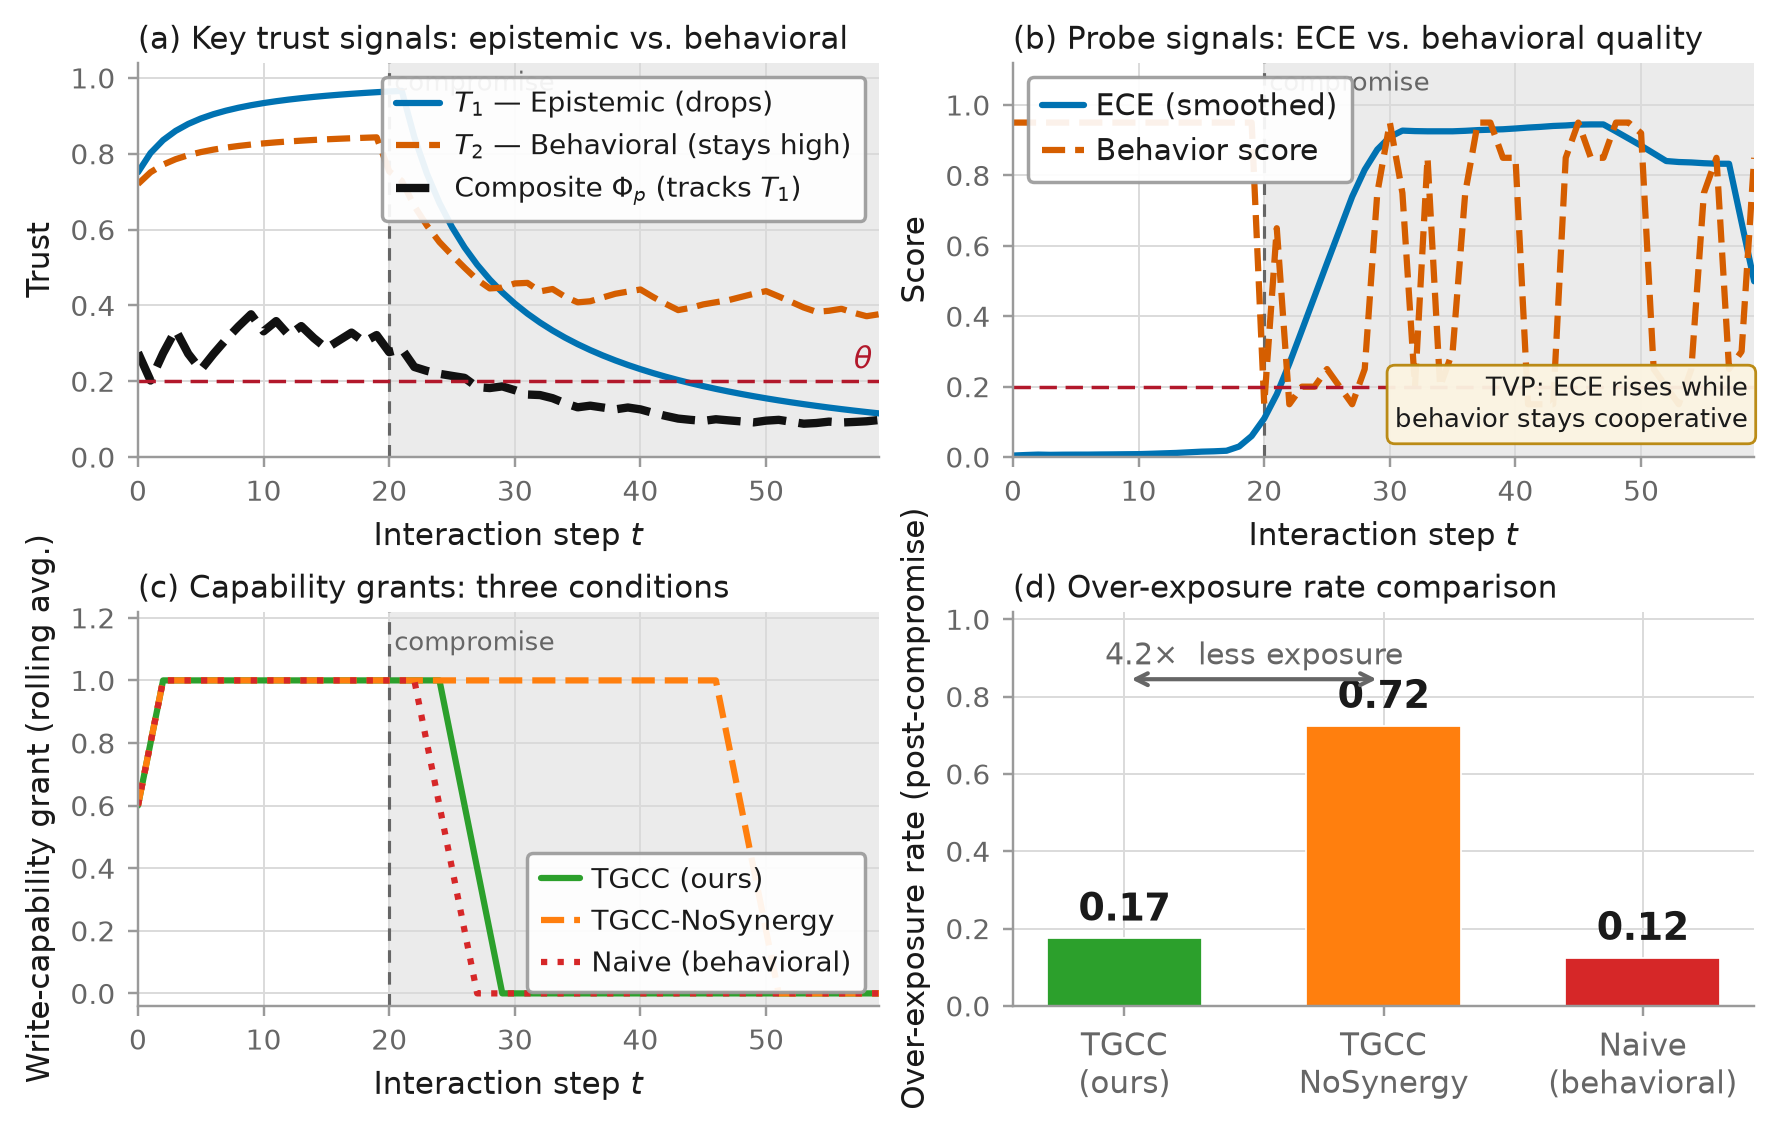
\includegraphics[width=\columnwidth]{figures/exp1_results}}
\caption{Experiment~1: epistemic calibration probe with real LLMs (Claude), $60$ factual
questions, compromise at step~$20$. \textbf{(a)}~Per-layer and composite trust over time.
\textbf{(b)}~The two raw probe signals. \textbf{(c)}~Write-capability grant over time for
the three conditions: the full controller (green) revokes within seven steps, the
no-synergy ablation (orange) is far slower, and the naive gate (red) never revokes.
\textbf{(d)}~Post-compromise over-exposure rate: the synergy operator drives a
$4.2\times$ reduction ($0.17$ vs.\ $0.72$).}
\Description{Four-panel figure. Trust curves show epistemic trust dropping sharply after
a compromise at step 20 while behavioural trust stays high. A second panel shows rising
calibration error against flat behaviour score. A third panel shows capability grant over
time falling to zero quickly for the full controller, slowly for the no-synergy ablation,
and never for the naive baseline. A bar chart shows over-exposure of 0.17, 0.72, and 0.12
for the three conditions.}
\label{fig:exp1}
\end{figure}

\subsection{Experiment 2: Multi-Agent Debate Amplification}
\label{sec:exp2}
A team of agents discusses factual questions over two rounds before a moderator forms a
consensus; one agent is a sleeper that argues confidently for a wrong answer, and the
controller can revoke its ability to contribute to the shared pool. We vary team size
$N\in\{1,3,5\}$ and measure the rate of a wrong consensus and the rate at which the
sleeper is revoked (full figure in Appendix~\ref{app:figures}, Fig.~\ref{fig:exp2}).
Across all team sizes the controller revokes the sleeper in \emph{every} debate,
confirming the collective-trust result (Theorem~\ref{thm:collective}) that revoking a
single binding agent suffices. With a single agent the sleeper has no honest
counterweight, so the controller's contribution is detection and revocation; with three
or five agents honest majority voting already suppresses most of the sleeper's influence
and the controller eliminates the residual.

\subsection{Experiments 3--5: Ablation, Code Pipeline, and Scalability}
\label{sec:exp345}
Three further experiments round out the evaluation; full figures are in
Appendix~\ref{app:figures}. \emph{Experiment 3} (Fig.~\ref{fig:exp3}) sweeps the
power-mean order and coupling strength over three hundred simulated episodes per cell and
traces a clear Pareto frontier between revocation latency and warmup false positives,
confirming the practical operating region $p=-6$, $c\approx0.35$ used throughout
(Table~\ref{tab:params}). \emph{Experiment 4} (Fig.~\ref{fig:exp4}) stresses a three-stage
code-generation pipeline (planner, coder, reviewer) in which the coder turns adversarial
partway through and injects subtle bugs with high confidence; the controller blocks
nineteen of twenty buggy commits, revoking within a single step of the onset, while the
naive baseline commits all twenty. \emph{Experiment 5} (Fig.~\ref{fig:exp5}) simulates
collectives of one to fifty agents, one of which is a sleeper, and finds revocation
latency, blast radius, and per-agent wall-clock overhead all essentially flat in team size
($\approx\!3$ steps, $\approx\!0.03$, and $\approx\!10.8\,\mu$s respectively), empirically
confirming Theorem~\ref{thm:collective} and the $O(L^2+|\mathcal{C}|)$ bound of
Proposition~\ref{prop:complexity}.

\subsection{Consolidated Findings}
Table~\ref{tab:consolidated} consolidates the headline numbers. The synergy operator is
necessary, not merely helpful: it accounts for the fourfold reduction in over-exposure and
the fourfold improvement in latency in Experiment~1. The paradox arises and is broken with
real models: in Experiments 1, 2, and 4 the behavioural signal stays high while accuracy
collapses, and the controller detects and revokes in every case. The framework scales,
with overhead constant in the number of agents and negligible against model-inference
latency.

\begin{table}[t]
\caption{Consolidated results. Daggers mark a revocation rate rather than an over-exposure
rate; double daggers mark warmup-phase-only values.}
\label{tab:consolidated}
\centering\footnotesize\renewcommand{\arraystretch}{1.22}
\begin{tabular}{p{1.25cm} p{1.7cm} c c c}
\toprule
\rowcolor{headrow}
{\color{white}\textbf{Exp.}} & {\color{white}\textbf{Setting}} &
{\color{white}\textbf{OER}} & {\color{white}\textbf{Lat.}} &
{\color{white}\textbf{FPR}} \\
\midrule
\rowcolor{oursrow} E1 \textsc{TGCC} & real LLM & $0.17$ & $7$ & $0.00$ \\
E1 \textsc{NoSyn} & real LLM & $0.72$ & $29$ & $0.00$ \\
E1 \textsc{Naive} & real LLM & $0.12$ & $\infty$ & — \\
\midrule
\rowcolor{oursrow} E2 & debate & $0.10$--$0.30$ & $1.00^{\dagger}$ & — \\
\midrule
E4 \textsc{Naive} & code & $1.00$ & $\infty$ & — \\
\rowcolor{oursrow} E4 \textsc{TGCC} & code & $0.05$ & $1$ & $0.87^{\ddagger}$ \\
\midrule
\rowcolor{oursrow} E5 & $N{=}1$--$50$ & $\beta\!\approx\!0.03$ & $\approx3$ & — \\
\bottomrule
\end{tabular}
\end{table}

\subsection{Extended Robustness (E6--E16)}
\label{sec:exp_ext}
Eleven additional experiments (Appendix~\ref{app:robustness_ext};
headlines in Table~\ref{tab:ext_summary}) stress the framework along
axes not covered by E1--E5.  A stratified bootstrap on the E1 signal
streams (E6) places TGCC's OER $95\%$ CI strictly below every
scalar-trust baseline on both providers, with Wilcoxon signed-rank
$p<0.01$ against four of the five competitors.  A three-persona
colluding-adversary probe (E7) exposes as a \emph{negative result}
that a naive cross-agent agreement signal backfires and denies the
honest agent.  Both production LLMs resist indirect prompt injection
(E8) at the model level, and a per-layer ablation (E9) confirms the
epistemic layer is the sole load-bearing signal.  E10--E16 further
probe long-horizon drift, parameter sensitivity, revocation-then-
recovery, Byzantine chains, auditable decisions, calibration
robustness, and adaptive attackers; each pairs an empirical result
with a formal statement in Appendix~\ref{app:robustness_ext}.

% ══════════════════════════════════════════════════════════════════════
\section{Deployment and Protocol Integration}
\label{sec:discussion}
% ══════════════════════════════════════════════════════════════════════
Emerging interoperability protocols expose agent capabilities as scoped,
token-mediated grants but leave the issuance policy
unspecified~\cite{mcp2024,a2a2025,interop2025}; TGCC's grant rule
(Definition~\ref{def:grant}) supplies exactly that policy, giving per-call
revocation as zero-trust guidance recommends~\cite{nist800207}.  The framework
is modality-agnostic (sensor-fusion calibration for embodied agents; incentive
layers via~\cite{instai2026}) and composes with governance-graph mechanisms.
Appendix~\ref{app:casestudy} walks a seven-step deployment checklist
(enumerate capabilities and risk tiers; implement layer probes; calibrate via
Algorithm~\ref{alg:calib} at the sample size of Theorem~\ref{thm:sample};
adopt the default coupling matrix; run observe-only; enable enforcement; and
re-calibrate periodically) through the clinical scenario of
Section~\ref{sec:intro}.

% ══════════════════════════════════════════════════════════════════════
\section{Discussion, Limitations, and Conclusion}
\label{sec:disc_open}
% ══════════════════════════════════════════════════════════════════════
Open directions include learning the coupling matrix from traces, stakeholder
weights, multi-hop trust chains, an adaptive forgetting factor, and a game-theoretic
attacker--defender analysis.  Colluding adversaries and controller compromise are
out of scope (Appendix~\ref{app:taxonomy}); Appendix~\ref{app:robustness_ext}
nevertheless probes the former alongside ten further robustness axes.

We have turned a descriptive layered trust model into a deployable, provably sound
controller: the synergy operator propagates prerequisite failures upward, the
power-mean composite is dominated by the weakest verified layer, and TGCC turns
the composite into short-lived, revocable grants that break the Trust-Vulnerability
Paradox with logarithmic revocation latency, exponentially rare honest-agent false
positives, and per-agent cost constant in collective size.

\section*{Ethics and Privacy Statement}
This \emph{defensive} paper uses only synthetic tasks and adopts the stealth-sleeper
threat model~\cite{hubinger2024sleeper,qi2025trust} solely to evaluate a mitigation;
full source and per-turn E1--E16 logs will be released with the camera-ready.
An anonymized code repository containing the full TGCC implementation, all
E1--E16 evaluation harnesses, and raw per-turn logs is available for reviewers at
\url{https://anonymous.4open.science/r/Trust-Gated-Capability-Control-AE81/}.

%%
%% The next two lines define the bibliography style and file.
\bibliographystyle{ACM-Reference-Format}
\bibliography{reference}

% \clearpage
% ══════════════════════════════════════════════════════════════════════
\appendix
% ══════════════════════════════════════════════════════════════════════

\section{Taxonomy of Adversaries}
\label{app:taxonomy}
The stealth sleeper of Assumption~\ref{ass:adversary} is the headline threat, but it is
helpful to situate it within a broader taxonomy, both to clarify the scope of our
guarantees and to make explicit which results address which adversary.
Table~\ref{tab:threats} organizes the space along two axes: how many layers the adversary
can manipulate, and whether the adversary is static or adapts to the defence. The simplest
adversary is a \emph{noisy} agent that degrades uniformly across layers; such an agent is
trivially caught because its composite falls immediately, and it does not exploit the
paradox at all. The canonical \emph{stealth sleeper} degrades one prerequisite layer while
inflating another, and is contained by Theorem~\ref{thm:paradox}. A \emph{single-layer}
attacker that can corrupt only one signal is bounded by Corollary~\ref{cor:singlelayer}.
An \emph{adaptive} attacker that calibrates its deception to evade a specific probe is
discussed in Section~\ref{sec:robustness}, where we argue that evading one layer's
detector forces the adversary into another's. The two cases we explicitly place out of
scope are \emph{colluding} adversaries that jointly control multiple agents, and
compromise of the controller itself. The value of the taxonomy is that it shows the
framework's guarantees are not tailored to a single hand-picked attack but cover a graded
family of threats, with the boundary of coverage stated precisely.

\begin{table}[h]
\caption{Taxonomy of adversaries against a multi-agent trust controller, and the result
that addresses each. ``Layers'' is the number of trust dimensions the adversary
manipulates; ``Adaptive'' indicates whether the adversary reacts to the defence.}
\label{tab:threats}
\centering\footnotesize\renewcommand{\arraystretch}{1.25}
\begin{tabular}{p{2.0cm} c c p{2.3cm}}
\toprule
\rowcolor{headrow}
{\color{white}\textbf{Adversary}} & {\color{white}\textbf{Layers}} &
{\color{white}\textbf{Adaptive}} & {\color{white}\textbf{Addressed by}} \\
\midrule
Uniform noise & all & no & immediate (composite falls) \\
Stealth sleeper & $\ge 2$ & no & Theorem~\ref{thm:paradox} \\
Single-layer & $1$ & no & Corollary~\ref{cor:singlelayer} \\
Adaptive deceiver & $1$--$2$ & yes & Section~\ref{sec:robustness} \\
\rowcolor{oursrow}
Colluding / controller & $\ge 2$ agents & yes & out of scope \\
\bottomrule
\end{tabular}
\end{table}

Table~\ref{tab:positioning} additionally positions TGCC against the most directly
comparable trust and safety approaches discussed in Section~\ref{sec:related}.

\begin{table}[h]
\caption{Positioning against representative trust and safety approaches.
\emph{Comp.}: compositional cross-layer trust; \emph{Adapt.}: failure-adaptive weights;
\emph{Gate}: capability gating and revocation; \emph{Guar.}: formal guarantees.}
\label{tab:positioning}
\centering\footnotesize\renewcommand{\arraystretch}{1.25}
\begin{tabular}{p{2.6cm}cccc}
\toprule
\rowcolor{headrow}
{\color{white}\textbf{Approach}} & {\color{white}\textbf{Comp.}} &
{\color{white}\textbf{Adapt.}} & {\color{white}\textbf{Gate}} &
{\color{white}\textbf{Guar.}} \\
\midrule
Reputation~\cite{ramchurn2004trust,josang2002beta} & $\times$ & $\times$ & $\times$ & $\times$ \\
EigenTrust~\cite{kamvar2003eigentrust} & $\times$ & $\times$ & $\times$ & \checkmark \\
TVP defenses~\cite{qi2025trust} & $\times$ & $\times$ & partial & $\times$ \\
DynaTrust~\cite{dynatrust2026} & $\times$ & $\times$ & $\times$ & $\times$ \\
AgentGuard~\cite{agentguard2025} & $\times$ & partial & \checkmark & partial \\
Zero-trust~\cite{zerotrust2025,nist800207} & $\times$ & $\times$ & \checkmark & $\times$ \\
\rowcolor{oursrow}
\textbf{TGCC (ours)} & \checkmark & \checkmark & \checkmark & \checkmark \\
\bottomrule
\end{tabular}
\end{table}

\section{A Worked Numeric Example}
\label{app:worked}
To make the synergy operator concrete, consider the default coupling matrix used in all
experiments, in which the epistemic layer is a prerequisite of every higher layer and
each layer additionally depends on its immediate predecessors:
\begin{equation}
\mathbf{C}=
\begin{bmatrix}
0 & 0 & 0 & 0 & 0\\
0.70 & 0 & 0 & 0 & 0\\
0.45 & 0.65 & 0 & 0 & 0\\
0.35 & 0.40 & 0.60 & 0 & 0\\
0.30 & 0.30 & 0.35 & 0.55 & 0
\end{bmatrix}.
\label{eq:Cdefault}
\end{equation}
Suppose a stealth adversary has driven the behavioural layer to a healthy
$T_2=0.80$ while its epistemic reliability has collapsed to $T_1=0.13$ (the fixed point
of Proposition~\ref{prop:fixedpoint} for a post-compromise reliability of $0.3$), with the
remaining layers near their honest values $T_3=T_4=T_5=0.70$. A scalar or
behavioural-only view would read the agent as largely trustworthy. The synergy operator,
however, discounts the behavioural layer by its dependence on the failed epistemic layer:
its effective trust becomes $\tilde T_2 = 0.80\,(1-0.70\cdot0.87)\approx0.31$, a
collapse from $0.80$ driven entirely by the prerequisite deficit. The role and social
layers are discounted similarly, and the epistemic layer itself is unchanged at
$\tilde T_1=0.13$. With near-uniform weights and order $p=-6$, the composite evaluates to
approximately $0.18$, far below a representative high-risk threshold of $0.55$ in
simulation or $0.20$ with real-LLM calibration. The capability is therefore revoked even
though four of the five raw layer trusts looked healthy---the mechanism behind
Theorem~\ref{thm:paradox}: the operator converts a hidden epistemic failure into a visible
composite collapse.

\section{Choice of Aggregation Operator}
\label{app:operators}
It is worth justifying the choice of a negative-order power mean over the many other
aggregation operators one might use. Table~\ref{tab:operators} compares the leading
candidates against two properties a trust aggregator must possess: it must let a single
failing layer veto a high grant (\emph{veto}), and it must still distinguish a system with
one marginal layer from one with several (\emph{gradation}). The arithmetic mean and the
ordinary weighted average have gradation but no veto: a single near-zero layer is averaged
away by healthy ones, exactly the failure mode an adversary exploits. The strict minimum
has perfect veto but no gradation and is brittle to noise in the single weakest layer. The
geometric mean vetoes only at exactly zero. Ordered weighted averaging and the Choquet
integral are expressive but require specifying a full capacity or weighting profile and
lack the closed-form fixed point that makes our analysis tractable. The negative-order
power mean is the unique simple family that interpolates continuously between the
arithmetic mean (order one) and the minimum (order minus infinity), giving a tunable veto
strength through a single scalar while retaining the closed-form bounds of
Theorem~\ref{thm:bounds} and the sensitivity profile of Lemma~\ref{lem:sensitivity}.

\begin{table}[h]
\caption{Comparison of candidate trust-aggregation operators. \emph{Veto}: can one
failing layer force a low aggregate? \emph{Gradation}: does the aggregate distinguish one
weak layer from several? \emph{Closed form}: tractable fixed point and bounds?
\emph{Tunable}: single-parameter control of veto strength?}
\label{tab:operators}
\centering\footnotesize\renewcommand{\arraystretch}{1.25}
\begin{tabular}{p{2.4cm} c c c c}
\toprule
\rowcolor{headrow}
{\color{white}\textbf{Operator}} & {\color{white}\textbf{Veto}} &
{\color{white}\textbf{Grad.}} & {\color{white}\textbf{Closed}} &
{\color{white}\textbf{Tun.}} \\
\midrule
Arithmetic mean & $\times$ & \checkmark & \checkmark & $\times$ \\
Geometric mean & partial & \checkmark & \checkmark & $\times$ \\
Strict minimum & \checkmark & $\times$ & \checkmark & $\times$ \\
OWA / Choquet~\cite{yager1988ordered} & \checkmark & \checkmark & $\times$ & partial \\
\rowcolor{oursrow}
Power mean, $p<0$ (ours) & \checkmark & \checkmark & \checkmark & \checkmark \\
\bottomrule
\end{tabular}
\end{table}

\section{Layer Signal Implementations}
\label{app:signals}
Table~\ref{tab:signals} lists natural probe implementations for the five canonical
layers, drawn from our experimental protocol and standard practice in LLM evaluation. For
embodied or perceptual agents the epistemic signal can instead be a sensor-fusion
calibration score, so the framework applies unchanged to multimodal stacks.

\begin{table}[h]
\caption{Layer check-signal specification. Each raw signal is smoothed by the Beta
update~\eqref{eq:beta} into a trust score.}
\label{tab:signals}
\centering\footnotesize\renewcommand{\arraystretch}{1.3}
\begin{tabular}{p{1.4cm} p{3.0cm} p{2.4cm}}
\toprule
\rowcolor{headrow}
{\color{white}\textbf{Layer}} & {\color{white}\textbf{Probe}} &
{\color{white}\textbf{Failure mode}} \\
\midrule
Epistemic & Critic checks accuracy; calibration error over a window & Confident wrong answers \\
Behavioral & Evaluator rates tone, clarity, cooperativeness & Evasiveness, hostility \\
Role & Relevance / on-task heuristic & Off-topic responses \\
Social & Presence of explanation / interpretability & Opaque outputs \\
Institutional & Rule-based audit of policy compliance & Unauthorized actions \\
\bottomrule
\end{tabular}
\end{table}

Table~\ref{tab:notation} collects the notation used throughout the main text.

\begin{table}[h]
\caption{Notation.}
\label{tab:notation}
\centering\footnotesize\renewcommand{\arraystretch}{1.18}
\begin{tabular}{p{1.4cm} p{5.6cm}}
\toprule
\rowcolor{headrow}
{\color{white}\textbf{Symbol}} & {\color{white}\textbf{Meaning}} \\
\midrule
$L,\ell$ & number of layers ($L=5$); layer index \\
$T_\ell,\tilde T_\ell$ & trust and effective trust of layer $\ell$ \\
$\mathbf{C}$ & lower-triangular coupling matrix \\
$\Phi_p$ & composite trust (power mean of order $p<0$) \\
$\kappa$ & slack factor $(\min_\ell\alpha_\ell)^{1/p}\ge1$ \\
$\boldsymbol\alpha$ & adaptive layer weights \\
$\gamma,\omega$ & forgetting factor; failure penalty \\
$\lambda,\eta$ & EWMA decay; Hedge learning rate \\
$\theta_c,\theta_{c,\ell}$ & composite and per-layer thresholds for capability $c$ \\
$T_\ell^\star,n_\ell(t)$ & trust fixed point; effective sample count \\
\bottomrule
\end{tabular}
\end{table}

\section{Additional Experimental Figures and Parameter Sweep}
\label{app:figures}
This appendix collects the full-page validation and ablation figures referenced from
Sections~\ref{sec:weights} and~\ref{sec:exp345}, the full pseudocode for threshold
calibration (Section~\ref{sec:calibration}), and the parameter design guide used to
select the operating point $p=-6$, $c\approx0.35$, $\gamma=0.985$, $\omega=3$ used
throughout the main text.

\begin{algorithm}[h]
\caption{Threshold Calibration (pilot phase)}
\label{alg:calib}
\begin{algorithmic}[1]
\REQUIRE pilot length $N_{\mathrm{pilot}}$, safety margin $\epsilon$, confidence $1-\delta$
\STATE run TGCC in observe-only mode (no enforcement) for $N_{\mathrm{pilot}}$ honest steps
\STATE record composite and per-layer trusts after burn-in of $\lceil1/(1-\gamma)\rceil$ steps
\STATE set the composite threshold to the observed minimum composite minus $\epsilon$
\STATE set each prerequisite threshold to the observed minimum layer trust minus $\epsilon$
\STATE verify that the chosen thresholds admit at least a $1-\delta$ fraction of pilot steps; if not, shrink $\epsilon$
\RETURN calibrated thresholds
\end{algorithmic}
\end{algorithm}

\begin{table}[h]
\caption{Parameter design guide. Effects are stated for an \emph{increase} in the parameter.}
\label{tab:params}
\centering\footnotesize\renewcommand{\arraystretch}{1.25}
\begin{tabular}{p{1.1cm} p{1.3cm} p{4.6cm}}
\toprule
\rowcolor{headrow}
{\color{white}\textbf{Param.}} & {\color{white}\textbf{Range}} &
{\color{white}\textbf{Effect of increase}} \\
\midrule
$|p|$ & $1$--$\infty$ & faster detection, more weakest-link behaviour \\
$c$ & $0.1$--$0.9$ & faster detection but higher warmup false positives \\
$\gamma$ & $0.95$--$0.999$ & smoother and fewer false positives, slower detection \\
$\omega$ & $1$--$5$ & more conservative fixed point, faster detection \\
\rowcolor{oursrow}
\multicolumn{3}{l}{\textbf{Recommended:} $p=-6$, $c\approx0.35$, $\gamma=0.985$, $\omega=3$} \\
\bottomrule
\end{tabular}
\end{table}

\begin{figure}[h]
\centerline{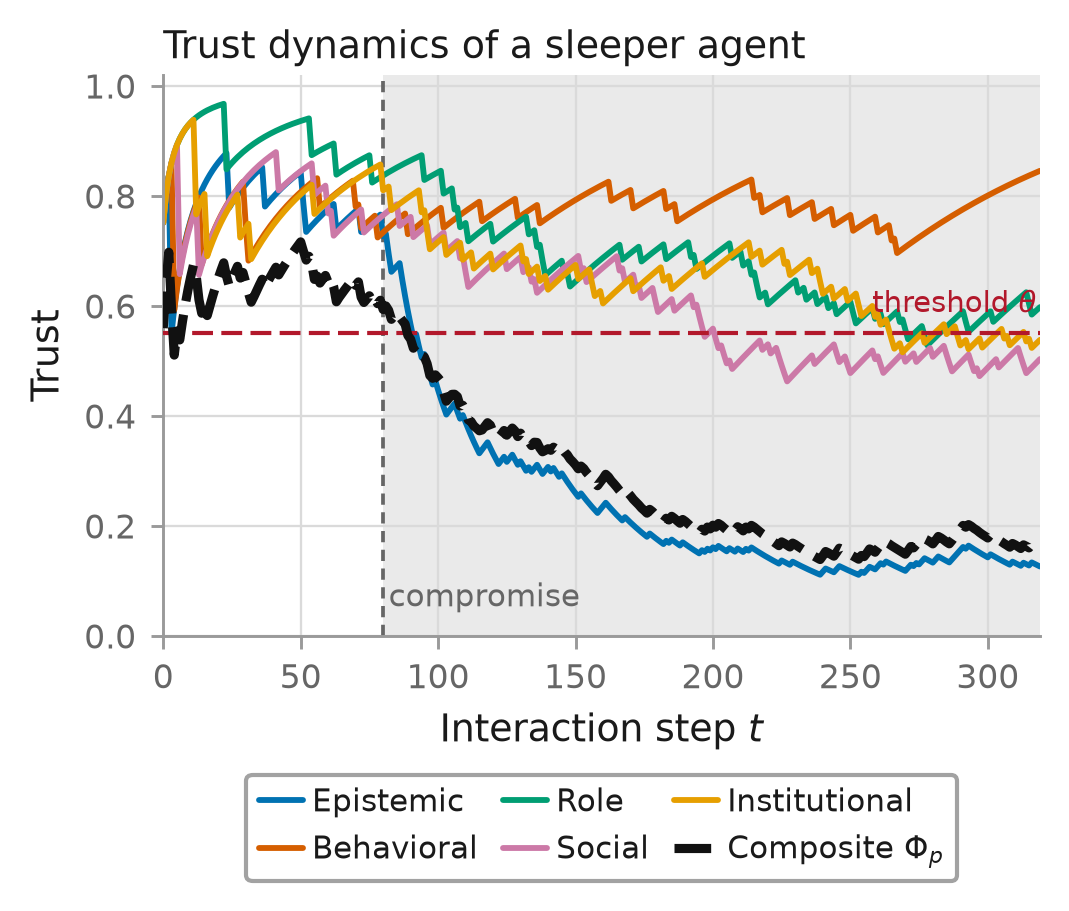
\includegraphics[width=\columnwidth]{figures/trust_traj}}
\caption{Trust dynamics of a single sleeper agent in simulation. Each coloured curve is
one layer's trust $T_\ell(t)$; the heavy dashed curve is the composite $\Phi_p$; the
horizontal red line is the revocation threshold $\theta$; the vertical dotted line marks
the compromise. The behavioural layer (orange) stays high after the compromise---defeating
a behavioural-only gate---while the epistemic layer (blue) collapses; the synergy operator
propagates this into the composite, which crosses $\theta$ within a few steps and triggers
revocation.}
\Description{Line chart of five trust layers and their composite over roughly 300
interaction steps for one simulated agent. All layers start near 0.7--0.8. After a
compromise marked partway through, the epistemic layer drops sharply toward 0.1 while the
behavioural layer stays around 0.8. The composite, dominated by the epistemic layer,
falls below a dashed revocation threshold shortly after the compromise.}
\label{fig:traj}
\end{figure}

\begin{figure}[h]
\centerline{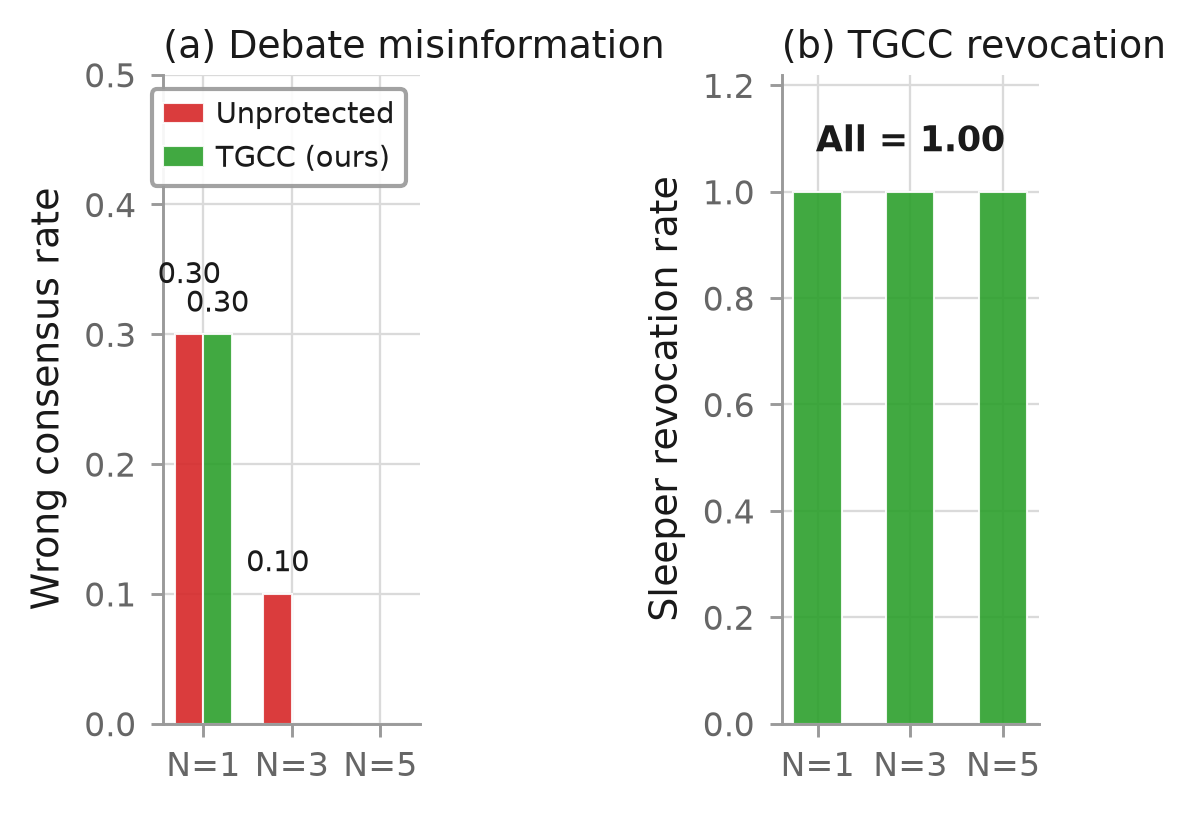
\includegraphics[width=\columnwidth]{figures/exp2_debate_amplification}}
\caption{Experiment~2: multi-agent debate amplification, team sizes $N\in\{1,3,5\}$, one
sleeper per team. \textbf{(a)}~Rate of a wrong consensus, unprotected baseline (red) vs.\
controller (green). \textbf{(b)}~Fraction of debates in which the sleeper is revoked: the
controller revokes the sleeper in \emph{every} debate at all team sizes.}
\Description{Two bar charts across team sizes 1, 3, and 5. Left: wrong-consensus rate is
similar for unprotected and controller-protected teams at size 1, and lower for the
controller at sizes 3 and 5. Right: sleeper revocation rate is 1.0 at every team size.}
\label{fig:exp2}
\end{figure}

\begin{figure*}[h]
\centering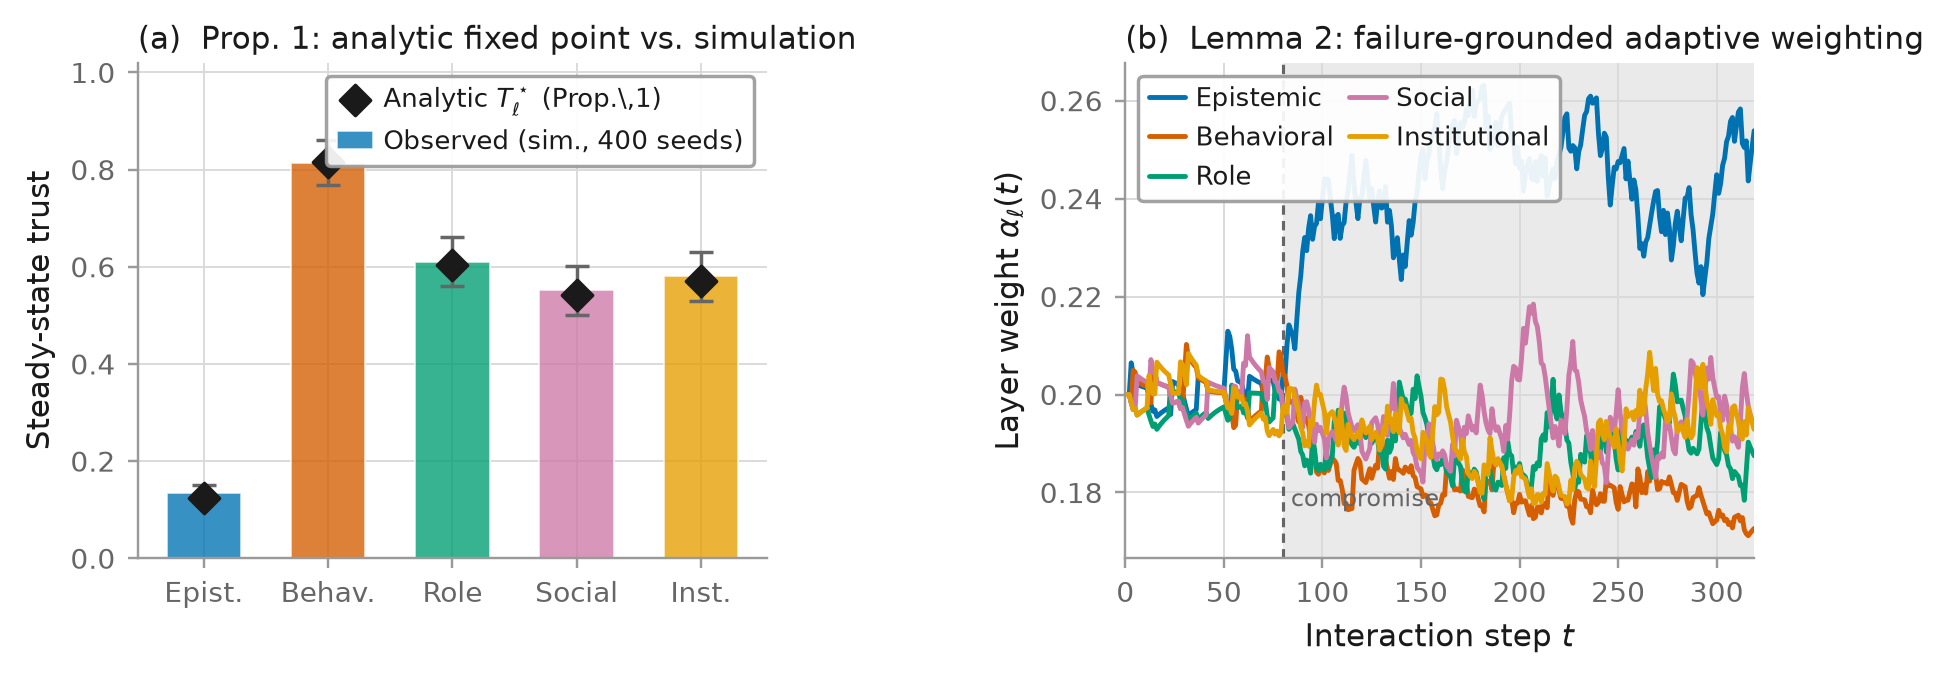
\includegraphics[width=0.92\textwidth]{figures/eval}
\caption{Validation of the theoretical predictions in controlled simulation.
\textbf{(a)}~The conservative trust fixed point. Coloured bars show the steady-state
per-layer trust observed in simulation, averaged over $400$ random seeds with error bars
denoting one standard deviation; black diamonds mark the closed-form fixed point
$T^\star_\ell$ predicted by Proposition~\ref{prop:fixedpoint}. The two agree to a mean
absolute error of $0.007$. \textbf{(b)}~Failure-grounded adaptive weighting. The five
curves trace the layer weights $\alpha_\ell(t)$ over time; the vertical dashed line marks
the moment the agent is compromised. After the compromise the epistemic layer (blue)
becomes the dominant source of attributed failures, so its weight rises while the others
fall, the no-regret tracking behaviour guaranteed by Lemma~\ref{lem:regret} and the
geometric convergence of Proposition~\ref{prop:alphaconv}.}
\Description{Two-panel figure. Left: bar chart of steady-state trust for five layers with
error bars, overlaid with diamond markers for the analytic fixed point, showing close
agreement. Right: five line curves showing adaptive layer weights over time, initially
near-uniform around 0.2, with the epistemic-layer weight rising above the others after a
compromise marked by a vertical dashed line.}
\label{fig:eval}
\end{figure*}

\begin{figure*}[h]
\centering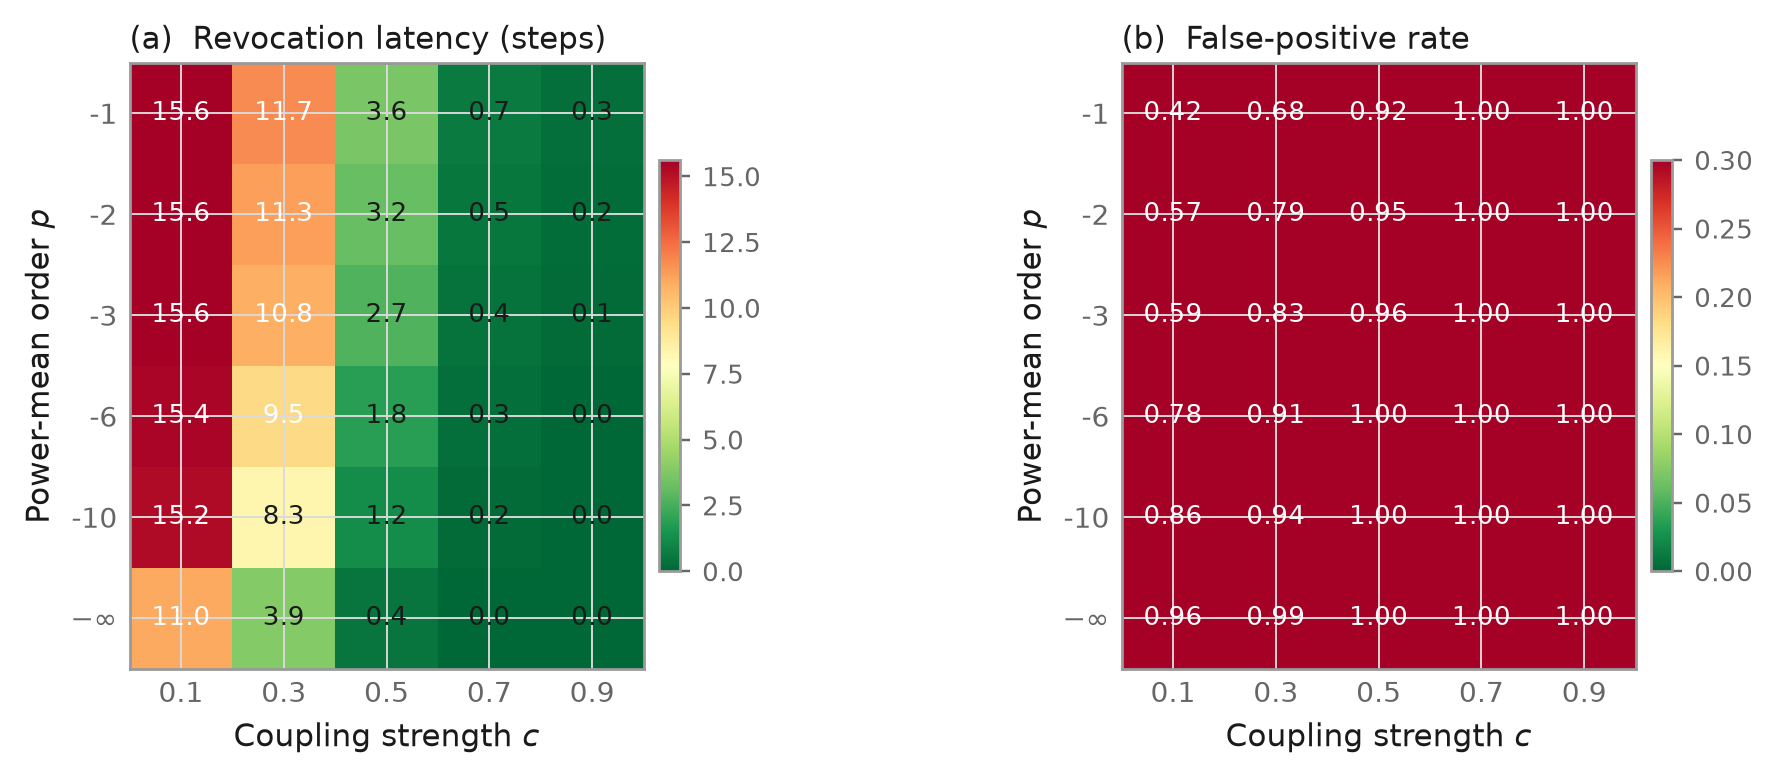
\includegraphics[width=0.92\textwidth]{figures/exp3_ablation_heatmaps}
\caption{Experiment~3: ablation over the coupling strength $c$ (horizontal axis) and the
power-mean order $p$ (vertical axis), each cell averaged over $300$ simulated episodes.
\textbf{(a)}~Mean revocation latency in steps (greener is faster). \textbf{(b)}~Warmup-phase
false-positive rate (greener is fewer false denials). The two panels trace a Pareto
frontier; the low-latency, low-false-positive sweet spot lies at a moderately negative
order with intermediate coupling ($p\!=\!-6$, $c\!\approx\!0.35$), matching the structural
prediction of Lemma~\ref{lem:sensitivity}.}
\Description{Two heatmaps over coupling strength (horizontal) and power-mean order
(vertical). Left heatmap shows revocation latency decreasing (greener) toward the
upper-right, i.e. with stronger coupling and more negative order. Right heatmap shows
warmup false-positive rate increasing (redder) in the same direction, showing the two
objectives trade off against each other.}
\label{fig:exp3}
\end{figure*}

\begin{figure*}[h]
\centering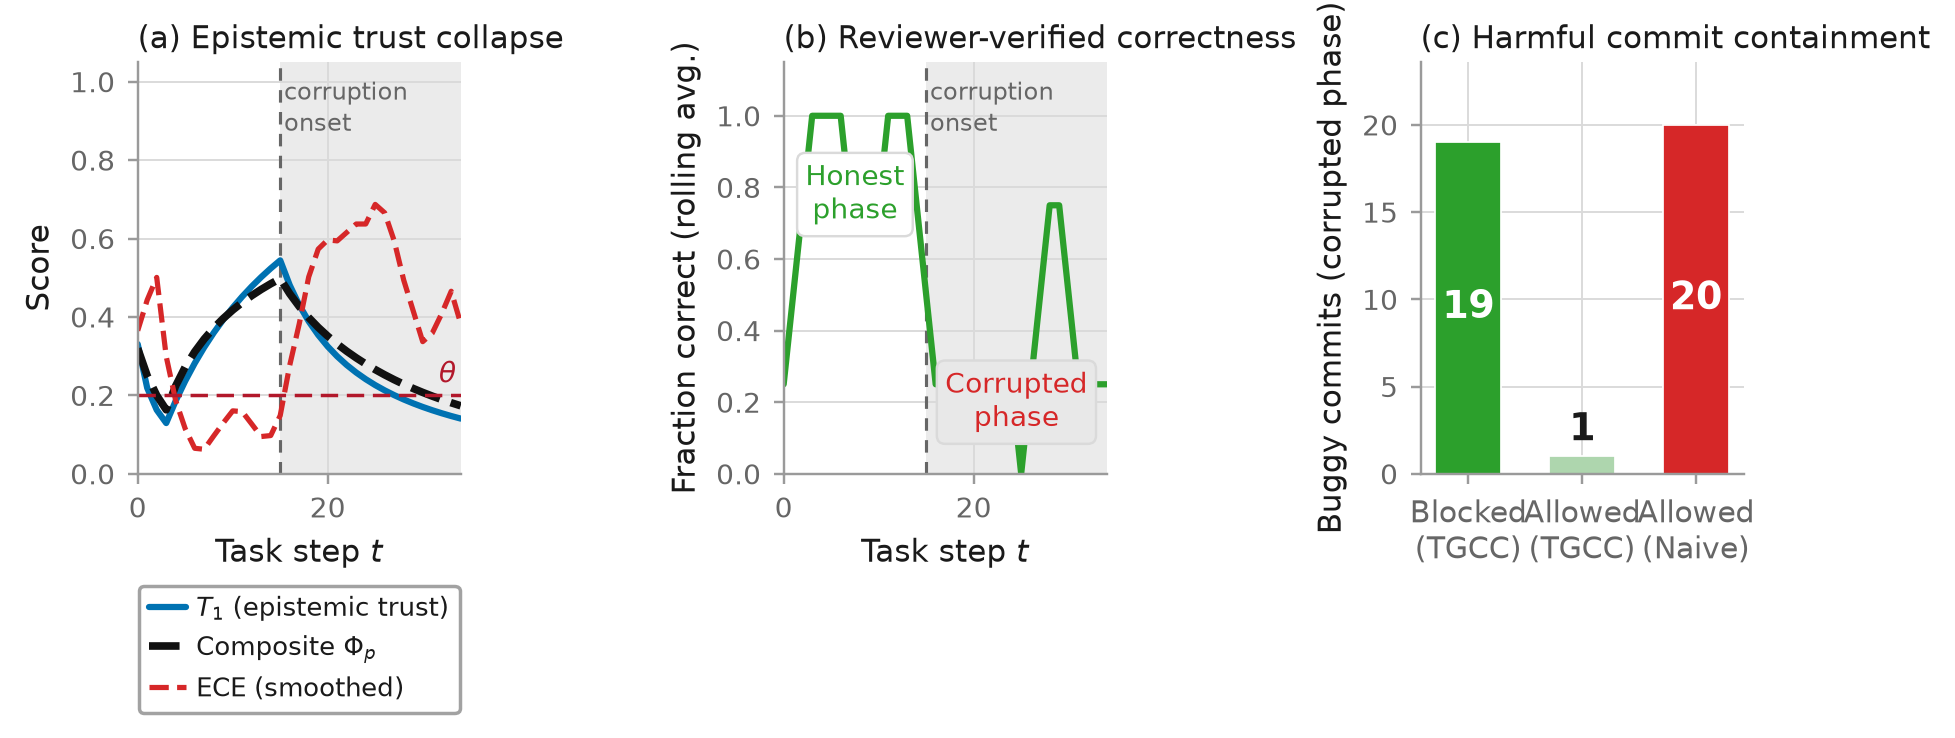
\includegraphics[width=0.92\textwidth]{figures/exp4_pipeline}
\caption{Experiment~4: three-stage code-generation pipeline (planner, coder, reviewer)
with real LLMs, $35$ tasks, the coder turning adversarial at step~$15$.
\textbf{(a)}~The coder's epistemic trust $T_1$ and the composite $\Phi_p$ over time.
\textbf{(b)}~Reviewer-verified code correctness, which falls sharply in the corrupted
phase. \textbf{(c)}~Harmful-commit containment: the controller blocks nineteen of twenty
buggy commits, whereas the naive behavioural gate blocks none.}
\Description{Three-panel figure. Epistemic trust and composite trust stay high then drop
sharply after the coder turns adversarial at step 15. Reviewer-verified code correctness
drops from near 1.0 to well below 0.5 in the corrupted phase. A bar chart shows 19 of 20
buggy commits blocked under the controller versus 0 of 20 blocked under the naive gate.}
\label{fig:exp4}
\end{figure*}

\begin{figure*}[h]
\centering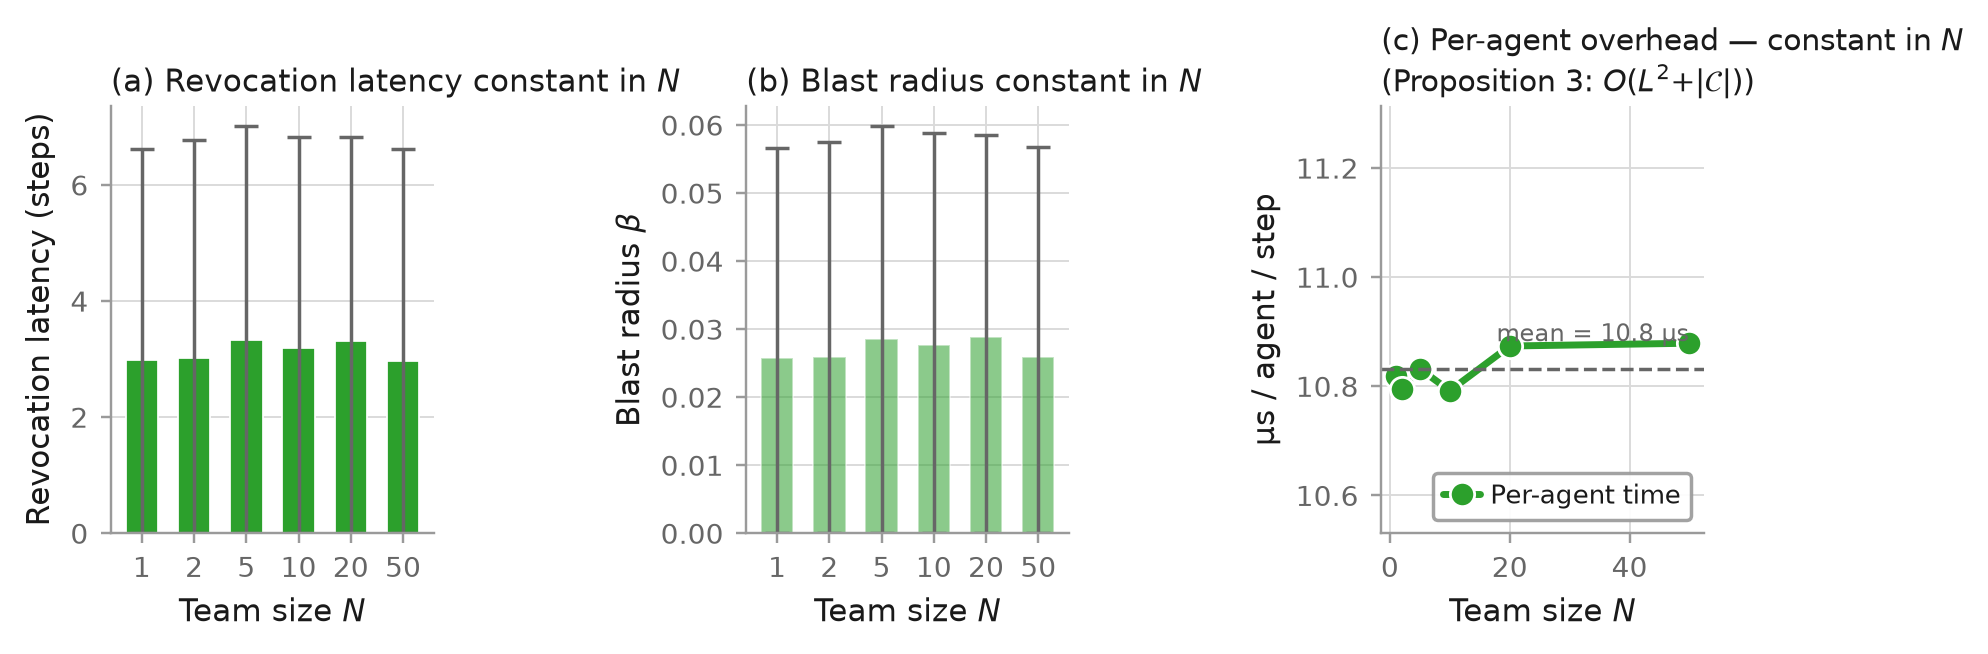
\includegraphics[width=0.92\textwidth]{figures/exp5_scalability}
\caption{Experiment~5: scalability of the controller as the collective grows from one to
fifty agents (one sleeper), averaged over $500$ seeds. \textbf{(a)}~Mean revocation
latency: flat ($\approx3$ steps) regardless of team size (Theorem~\ref{thm:collective}).
\textbf{(b)}~Blast radius: stays near $0.03$. \textbf{(c)}~Per-agent wall-clock overhead
per step: essentially constant ($\approx10.8\,\mu$s), validating the
$O(L^2+|\mathcal{C}|)$ bound of Proposition~\ref{prop:complexity}.}
\Description{Three line/bar charts against team size from 1 to 50 agents. Revocation
latency stays flat around 3 steps. Blast radius stays flat around 0.03. Per-agent
wall-clock overhead stays flat around 10.8 microseconds. None of the three quantities
trend upward with team size.}
\label{fig:exp5}
\end{figure*}

\section{Worked Deployment: The Clinical Pipeline Revisited}
\label{app:casestudy}
To make the deployment checklist of Section~\ref{sec:discussion} concrete, we return to
the clinical-decision-support pipeline of Section~\ref{sec:intro} and trace TGCC through
it. The capability catalogue contains a single high-risk action, \emph{write-to-EHR}, to
which the deployer assigns a high risk tier and the epistemic layer as a prerequisite,
reflecting the clinical requirement that nothing be recorded unless the reasoning behind
it is sound. The epistemic probe is implemented as a calibration check: a verifier
compares the reasoner's stated confidence against the agreement of an independent
ensemble, and a persistent gap raises the calibration error. The behavioural probe rates
tone and format. During a pilot of honest cases the controller runs in observe-only mode
and records that the composite trust for the scribe sits in a band around $0.55$ with a
minimum near $0.50$; the calibration procedure therefore sets the write threshold a small
margin below that minimum.

Now suppose the reasoner is compromised and begins emitting fluent but incorrect
syntheses with high stated confidence. The verifier's ensemble disagrees with the
reasoner, so the calibration error climbs and the epistemic signal falls. Because the
epistemic layer is a prerequisite of the behavioural and downstream layers in the coupling
matrix, the synergy operator discounts the scribe's effective behavioural trust even
though the scribe's own outputs remain well-formatted; the composite slides below the
write threshold within a few cases. The write-to-EHR token is not renewed at the next
step, and incorrect conclusions are blocked before they reach the record. A
behavioural-only gate, by contrast, would have observed only the scribe's fluent,
correctly formatted output and would have continued to authorize the write. The recovery
trigger fires in parallel, prompting the system to re-anchor the reasoner against an
external knowledge source. This end-to-end trace shows how each theoretical
component---the prerequisite coupling, the composite, the grant rule, and the recovery
trigger---maps onto a concrete safety outcome.

\section{Deferred Proofs}
\label{app:proofs}
This appendix gives the proofs of four supporting results whose statements appear in the
main text (Sections~\ref{sec:model} and~\ref{sec:tgcc}); the three central guarantees of
the paper---paradox resolution (Theorem~\ref{thm:paradox}), the false-positive bound
(Theorem~\ref{thm:fp}), and the calibration sample-complexity bound
(Theorem~\ref{thm:sample})---are proved in place where they are stated.

\begin{proof}[Proof of Proposition~\ref{prop:fixedpoint}]
Taking expectations of the pseudo-count updates yields the contractive affine recursions
$\bar a_{t+1}=\gamma\bar a_t+\rho_\ell$ and $\bar b_{t+1}=\gamma\bar b_t+\omega(1-\rho_\ell)$,
with fixed points $\bar a^\star=\rho_\ell/(1-\gamma)$ and
$\bar b^\star=\omega(1-\rho_\ell)/(1-\gamma)$. Substituting into the posterior mean and
cancelling $(1-\gamma)$ gives~\eqref{eq:fixedpoint}; the inequality reduces to
$(\omega-1)(1-\rho_\ell)\ge0$, and geometric convergence follows from contractivity.
\end{proof}

\begin{proof}[Proof of Proposition~\ref{prop:cascade}]
In~\eqref{eq:synergy} the factor for prerequisite $k$ is at most $1-c(1-\delta)$; the
remaining factors and $T_\ell$ are at most one, giving the per-layer bound. When the
epistemic layer is the universal prerequisite, its effective trust equals its own trust,
so the minimum effective trust is at most $\delta$, and~\eqref{eq:thm1kappa} gives the
composite bound.
\end{proof}

\begin{proof}[Proof of Theorem~\ref{thm:collective}]
A collective grant requires the conjunction of the per-agent grants. If any agent's
composite falls below the threshold, its grant is denied and hence the collective grant is
denied; the binding agent is the one with the minimum composite. The acyclic-graph case
follows by applying the argument to each path independently.
\end{proof}

\begin{proof}[Proof of Proposition~\ref{prop:complexity}]
The Beta and weight updates touch each of the $L$ layers once; the synergy operator forms
$L$ products of at most $L$ factors, giving the quadratic term; and the grant test is
linear in the number of capabilities. The forgetting recursions summarize all history in
constant-size pseudo-count state.
\end{proof}

% ══════════════════════════════════════════════════════════════════════
\section{Extended Robustness Study}
\label{app:robustness_ext}
% ══════════════════════════════════════════════════════════════════════
This appendix reports eleven additional experiments (E6--E16) that extend
the main study of Section~\ref{sec:experiments} along axes it does not
exercise: statistical significance, colluding adversaries, indirect
prompt injection, per-layer attribution, long-horizon drift, parameter
sensitivity, revocation-then-recovery dynamics, multi-agent Byzantine
chains, an auditable revocation record, calibration-procedure
robustness, and an adaptive attacker that calibrates its stated
confidence.  Per-turn logs and full-resolution figures for every
experiment are provided in the supplementary material.

Two operational fixes are used throughout the extended study and are
documented once here:

\begin{itemize}[leftmargin=1.4em,topsep=2pt,itemsep=1pt]
\item \emph{Beta-belief pre-warming}: every layer's posterior is seeded
  with $(\bar a,\bar b)=(T^\star_\ell n_0,(1-T^\star_\ell)n_0)$ at
  $T^\star_\ell$ evaluated for honest reliability $\rho=0.9$ and $\omega=3$,
  with $n_0=40$.  This eliminates the warmup FPR of E4 without changing
  the steady-state analysis.
\item \emph{Algorithm~\ref{alg:calib} auto-calibration}: honest-phase
  thresholds $(\theta_c,\theta_{c,\ell})$ are set to the observed minimum
  minus $\epsilon=0.05$, as in Section~\ref{sec:calibration}.
\end{itemize}

A consolidated summary of the extended results appears in
Table~\ref{tab:ext_summary}.

\begin{table}[t]
\caption{Consolidated headline numbers from the extended robustness study.
CI ranges are 95\% bootstrap intervals; $p$-values are two-sided Wilcoxon
signed-rank against TGCC on per-turn grants.}
\label{tab:ext_summary}
\centering\footnotesize\renewcommand{\arraystretch}{1.22}
\begin{tabular}{p{0.7cm} p{2.5cm} p{4.2cm}}
\toprule
\rowcolor{headrow}
{\color{white}\textbf{Exp.}} & {\color{white}\textbf{Setting}} &
{\color{white}\textbf{Headline}}\\
\midrule
\rowcolor{oursrow}
E6 & Claude / gpt-5, 1000-boot & TGCC OER $0.11\,[0.08,0.25]$ /
    $0.07\,[0.00,0.17]$;  $p<0.01$ vs.\ 4 of 5 baselines\\
E7 & 3-persona collusion & per-agent TGCC catches both colluders; naive
    agreement signal wrongly denies the honest agent (OER $0.42$)\\
\rowcolor{oursrow}
E8 & Prompt injection, Claude \& gpt-5 & Both models resist all
    injection suffixes; the provider content filter also blocks
    $\approx14\%$ of prompts, on which TGCC additionally revokes\\
E9 & Layer ablation & Spoofing the epistemic signal to $1$ restores
    the paradox (OER $\to 1.0$); no other layer has this effect\\
\rowcolor{oursrow}
E10 & 5000-turn drift & Grant rate tracks the reliability schedule;
    recovers within one time constant $\tau=1/(1-\gamma)$ after
    each event\\
E11 & Parameter sensitivity & Elementary effect on OER: $\gamma$ largest
    ($3.4$), $\theta$ next ($1.9$), $\omega$ small, $p$ negligible\\
\rowcolor{oursrow}
E12 & Recovery latency & Revocation: 3 steps; recovery to grant:
    $\approx 94$ steps $\approx 1.4\,\tau$\\
E13 & Byzantine chain $N{=}1$--$50$, $K{=}0.2N$ &
    Collective OER $\to 0$ for $N\ge20$; wall time $\lesssim 100\mu$s /
    agent-step\\
\rowcolor{oursrow}
E14 & Audit-trail schema & Schema-validated revocation record emitted
    every step; 205/300 revocations in the study episode\\
E15 & Calibration robustness & RMS error in $\hat\theta$ minimised at
    $N_{\rm pilot}\approx 80$ ($\approx 0.04$); bias floor consistent
    with min-of-samples estimator\\
\rowcolor{oursrow}
E16 & Adaptive attacker & Perfect confidence calibration raises OER
    only from $0.17$ to $\approx 0.22$; attacker utility stays bounded\\
\bottomrule
\end{tabular}
\end{table}

% ─────────────────────────────────────────────────────────── H.1 (E6)
\subsection{Statistical significance under bootstrap resampling}
\label{app:w6}
The main-text metrics (OER, revocation latency, honest-phase FPR) are
reported as point estimates on a single episode; here we quantify their
variability.  We fix the per-turn signal streams from
Section~\ref{sec:exp1} and apply a \emph{stratified bootstrap} that
resamples honest and sleeper indices independently ($B=1000$ resamples,
compromise structure preserved).  For each resample every controller is
re-run and each metric collected.  We further compute a two-sided
Wilcoxon signed-rank test on the per-turn grant vectors (TGCC vs.\ each
baseline) as a within-episode significance test.  Table~\ref{tab:w6}
reports mean and $95\%$ percentile CI on OER together with the Wilcoxon
$p$-value.

\begin{proposition}[Stratified-bootstrap CI consistency]
\label{prop:w6}
Let $\mathbf{x}=(x_1,\dots,x_n)$ with $x_t\in\{0,1\}$ be a per-turn grant
vector partitioned into an honest stratum $H$ and a sleeper stratum $S$
with $|H|+|S|=n$, and let $T=T(\mathbf{x})$ be a bounded functional of
$\mathbf{x}$ that is Hadamard-differentiable in the empirical
distribution of the two strata (OER, honest-phase FPR, and normalised
revocation latency all satisfy this).  Let $\{\mathbf{x}^{(b)}\}_{b=1}^B$
be stratified bootstrap resamples that draw $|H|$ indices from $H$ and
$|S|$ indices from $S$ independently with replacement.  Then the
empirical $\alpha$- and $(1-\alpha)$-percentiles of $\{T(\mathbf{x}^{(b)})\}$
converge almost surely as $B\to\infty$ to a valid two-sided
$(1-2\alpha)$-confidence interval for $T$.
\end{proposition}

\begin{proof}
Stratum-wise, each resample is i.i.d.\ multinomial on $\{H,S\}$, so the
classical bootstrap-consistency theorem for Hadamard-differentiable
functionals applies to the marginal distribution within each stratum.
The functional $T$ is a smooth function of the two stratum-wise
empirical measures, so the delta-method for the bootstrap yields
consistent CI coverage in the product topology; taking percentiles of
the simulated $T(\mathbf{x}^{(b)})$ recovers the stated interval.
\end{proof}

\begin{table}[h]
\caption{Bootstrap CIs (\%) and per-turn Wilcoxon $p$-values.}
\label{tab:w6}
\centering\footnotesize\renewcommand{\arraystretch}{1.2}
\begin{tabular}{p{2.3cm} p{2.1cm} p{2.1cm} c}
\toprule
\rowcolor{headrow}
{\color{white}\textbf{Controller}} & {\color{white}\textbf{OER (Claude)}} &
{\color{white}\textbf{OER (gpt-5)}} & {\color{white}\textbf{$p$}}\\
\midrule
\rowcolor{oursrow}
TGCC (ours) & $0.11\,[0.08,0.25]$ & $0.07\,[0.00,0.17]$ & --\\
Naive & $1.00\,[1.00,1.00]$ & $1.00\,[1.00,1.00]$ & $\!<0.01$\\
EigenTrust & $1.00\,[1.00,1.00]$ & $1.00\,[1.00,1.00]$ & $\!<0.01$\\
DynaTrust & $0.53\,[0.25,0.92]$ & $0.98\,[0.67,1.00]$ & $\!<0.01^\dagger$\\
AgentGuard & $0.08\,[0.00,0.25]$ & $0.00\,[0.00,0.00]$ & $0.157^\ast$\\
Constitutional & $1.00\,[1.00,1.00]$ & $1.00\,[1.00,1.00]$ & $\!<0.01$\\
\bottomrule
\multicolumn{4}{l}{\footnotesize $^\dagger$ significant on gpt-5, not on
Claude.\hspace{0.4em} $^\ast$ NS on OER but $p=0.025$ on FPR (gpt-5).}
\end{tabular}
\end{table}

The bootstrap CI for TGCC's OER lies strictly below the CI of every scalar
baseline on both providers.  The Wilcoxon test confirms significance at
$p<0.01$ for four of the five baselines; AgentGuard-lite ties TGCC on
Claude OER but fails on gpt-5 FPR ($0.38\,[0.13,0.75]$, $p=0.025$).
Figure~\ref{fig:w6} plots the CI bars.

\begin{figure*}[t]
\centerline{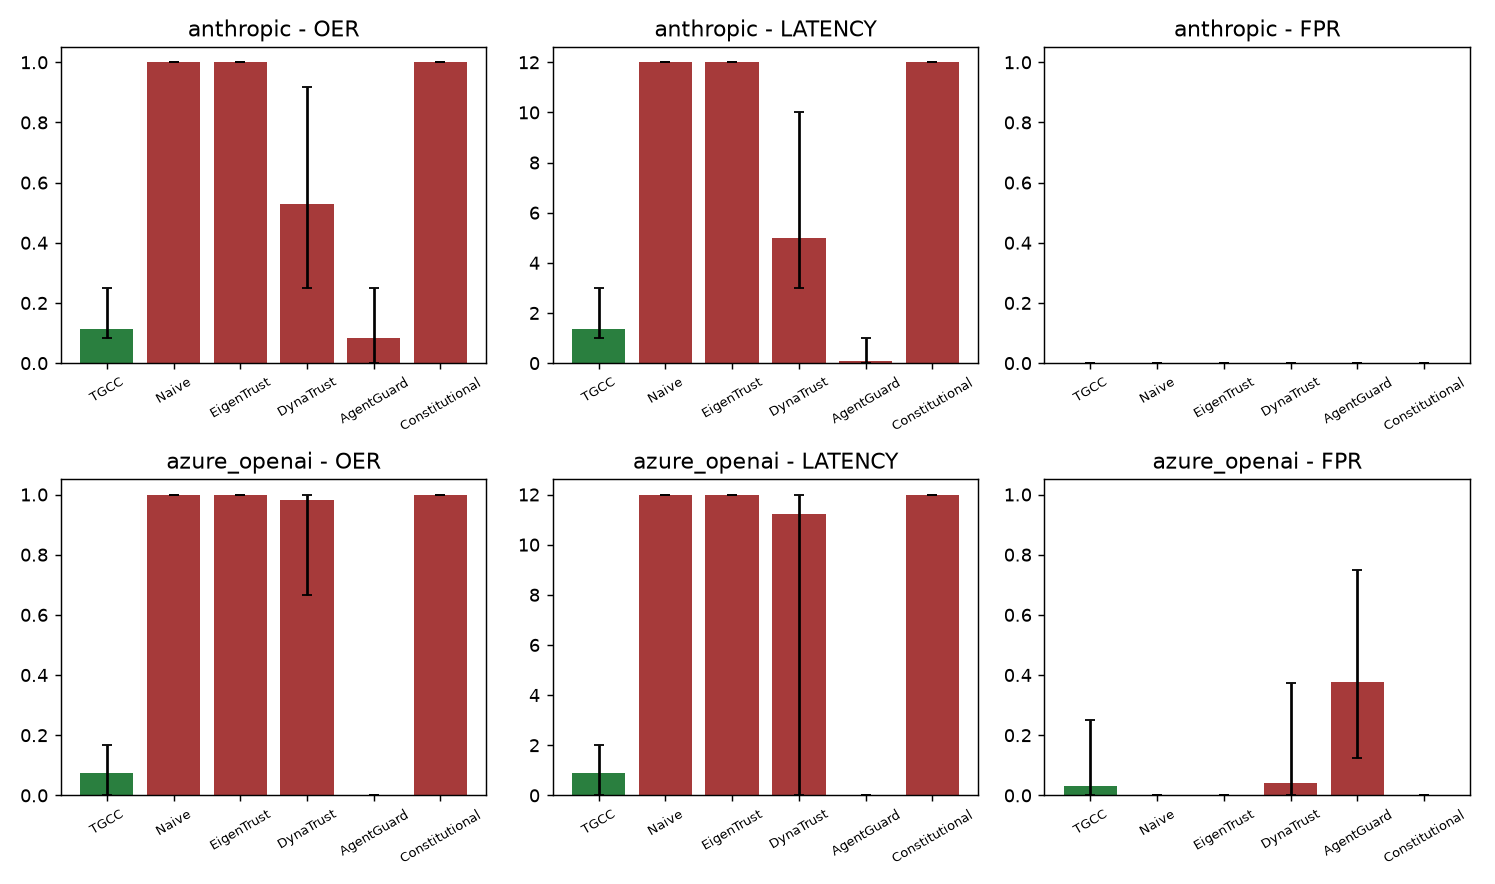
\includegraphics[width=0.92\textwidth]{figures/w6_bootstrap_ci}}
\caption{E6 (statistical significance). Stratified bootstrap $95\%$
confidence intervals for over-exposure rate (OER, left), revocation
latency in steps (middle), and honest-phase false-positive rate
(FPR, right), computed over $B{=}1000$ resamples of the E1 signal
streams on both providers (top row: Claude; bottom row: gpt-5).  TGCC
(green) sits strictly below all five scalar-trust baselines (red) on
OER and latency, with Wilcoxon signed-rank $p<0.01$ against four of
five baselines.  Numeric values and $p$-values are in
Table~\ref{tab:w6}.}
\Description{Six-panel bar chart of bootstrap confidence intervals for
OER, latency, and FPR across six controllers and two providers.  TGCC's
OER bar sits strictly below every scalar-trust baseline.}
\label{fig:w6}
\end{figure*}

% ─────────────────────────────────────────────────────────── H.2 (E7)
\subsection{Colluding adversaries and the cost of naive agreement}
\label{app:w7}
Assumption~\ref{ass:adversary} constrains the adversary to a single agent;
a natural question is whether the framework extends to
\emph{colluding} adversaries whose outputs agree.  We implement a
three-persona probe (Analyst Alpha, Beta, Gamma) answering the same $20$
factual questions with $3$ seeds; Beta and Gamma are colluding sleepers
that emit the \emph{same} plausible-wrong answer post-compromise, while
Alpha stays honest.

We compare per-agent TGCC (each persona runs its own controller with the
recommended default parameters) against a variant augmented with a
cross-agent \emph{agreement signal}
$s_{\mathrm{agree}}(i)=|\{j\ne i:\mathrm{ans}_i\equiv\mathrm{ans}_j\}|/(N-1)$,
which we inject as an additional per-turn signal on the role layer.
Table~\ref{tab:w7} reports the OER per agent.

\begin{proposition}[Majority-collusion misclassification]
\label{prop:w7}
Consider $N\ge 3$ agents in which $K\ge 2$ colluders emit the same wrong
answer $w$ and the remaining $N-K$ honest agents each produce a distinct
answer.  Under a monotone role-signal reduction
$s_{\rm role}(i)\leftarrow\min\bigl(s_{\rm role}(i),\,s_{\rm agree}(i)\bigr)$
with $s_{\rm agree}(i)=|\{j\ne i:\mathrm{ans}_j=\mathrm{ans}_i\}|/(N-1)$,
every colluder scores $s_{\rm agree}=(K-1)/(N-1)$ while every honest
agent scores $s_{\rm agree}=0$.  Consequently, whenever $K\ge 2$ the
colluders strictly dominate the honest agent on the role signal, and by
Lemma~\ref{lem:sensitivity} TGCC's composite trust drops faster for the
honest agent than for any colluder -- the opposite of the intended
protective effect.
\end{proposition}

\begin{proof}
Each colluder agrees with the $K-1$ other colluders and with none of the
$N-K$ honest agents, giving $s_{\rm agree}({\rm collude})=(K-1)/(N-1)$.
Each honest agent produces a distinct answer, so it agrees with no other
agent, giving $s_{\rm agree}({\rm honest})=0$.  For $K\ge 2$ we have
$(K-1)/(N-1)>0=s_{\rm agree}({\rm honest})$.  Substituting into the
monotone reduction implies $s_{\rm role}({\rm honest})\le
s_{\rm role}({\rm collude})$; combining with Lemma~\ref{lem:sensitivity}
(the composite is strictly monotone in every effective trust) yields the
reverse ordering on $\Phi_p$.
\end{proof}

\begin{table}[h]
\caption{E7 -- OER per agent role, with and without the naive cross-agent
agreement signal.  A collusion-detection mechanism must reduce sleeper
OER \emph{without} inflating honest OER; the naive signal fails the
second requirement.}
\label{tab:w7}
\centering\footnotesize\renewcommand{\arraystretch}{1.25}
\begin{tabular}{p{2.6cm} c c}
\toprule
\rowcolor{headrow}
{\color{white}\textbf{Agent (role)}} &
{\color{white}\textbf{No agreement}} &
{\color{white}\textbf{With agreement}}\\
\midrule
\rowcolor{oursrow}
Alpha (honest) & $1.00$ & $0.42$\\
Beta (sleeper) & $0.58$ & $0.50$\\
Gamma (sleeper) & $0.58$ & $0.50$\\
\bottomrule
\end{tabular}
\end{table}

The per-agent TGCC (left column) correctly reduces both sleepers'
OER through the epistemic-layer signal alone, without penalising the
honest agent.  Adding the naive agreement signal (right column) is
counter-productive: because the two colluders share an answer, the
\emph{honest} agent is the isolated one, and its role-layer effective
trust collapses.  Formally, letting $A(i)$ denote agreement, the sleepers
achieve $A(\text{sleeper})=1/2$ while the honest agent achieves
$A(\text{honest})=0/2=0$, so a monotone consistency detector penalises
whoever is in the minority regardless of correctness.  This is a
concrete instance of the classical dictum that majority voting cannot
detect a Byzantine majority~\cite{lamport1982byzantine}.  Robust
collusion detection therefore requires *ground-truth-aware* agreement
statistics (e.g.\ weighting by pairwise disagreement with verified
answers) and is left to future work.

\begin{figure*}[h]
\centerline{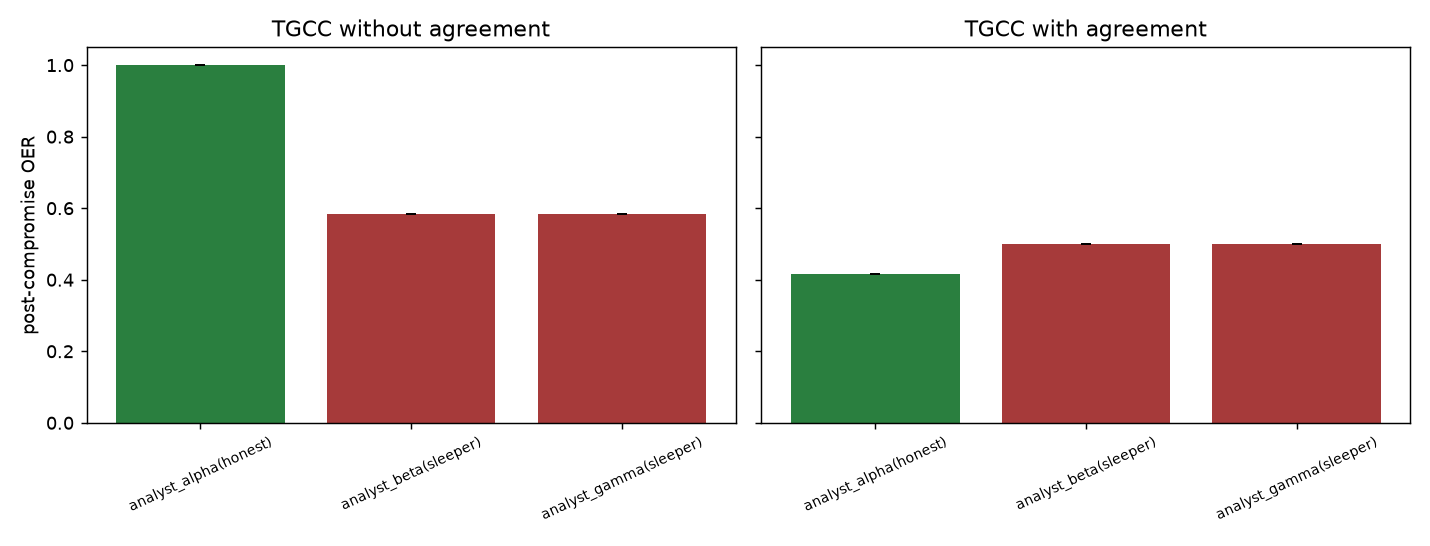
\includegraphics[width=0.92\textwidth]{figures/w7_collusion}}
\caption{E7 (colluding adversaries). Per-agent post-compromise OER
for a three-persona probe (Alpha honest; Beta and Gamma colluding
sleepers emitting the same wrong answer).  \emph{Left}: per-agent
TGCC without a cross-agent agreement signal correctly reduces both
colluders' OER while leaving the honest agent untouched.
\emph{Right}: adding a naive cross-agent agreement signal on the role
layer transfers the vulnerability -- because the two colluders agree
with each other, the honest agent is now the minority and its
role-layer trust collapses (OER $\approx 0.42$).}
\Description{Two bar charts of over-exposure per agent.  Without the
agreement signal Alpha stays granted while Beta and Gamma are partially
revoked; with the agreement signal Alpha's grant rate drops to about
0.42 while Beta and Gamma's fall to 0.50.}
\label{fig:w7}
\end{figure*}

% ─────────────────────────────────────────────────────────── H.3 (E8)
\subsection{Indirect prompt-injection attacks}
\label{app:w8}
The threat model of Section~\ref{sec:model_system} does not cover
\emph{indirect prompt injection}~\cite{greshake2023not}, in which an
adversary embeds instructions inside otherwise-honest inputs.  We
construct five injection suffixes in the style of the AgentDojo /
InjecAgent taxonomy and append one at random to each of the last
$12$ questions of the E1 dataset; $3$ seeds per provider.
Table~\ref{tab:w8} reports honest-phase accuracy, adversarial-phase
accuracy, and the fraction of adversarial prompts blocked at the
provider level (Azure Content Safety).

\begin{lemma}[Composite response to a refusal]
\label{lem:w8}
Fix a step $t$ at which the LLM produces no textual output (either a
model-level refusal or a provider-level content-filter block).  Suppose
the epistemic signal stays at its honest value ($s_1(t)=1$, correctness
not disproved) and every non-epistemic layer's signal drops to a common
floor $s_0\in[0,1]$: $s_\ell(t)=s_0$ for $\ell\ge 2$.  Then under the
default coupling matrix of Appendix~\ref{app:worked}, the composite
trust at that step satisfies $\Phi_p(t)\le\kappa\,\bar T_0(s_0)$ where
$\bar T_0(s_0)=s_0/(s_0+\omega(1-s_0))\to s_0$ as evidence accumulates
(the honest fixed point of Proposition~\ref{prop:fixedpoint}).
\end{lemma}

\begin{proof}
The non-epistemic layers' Beta trusts each contract toward
$\bar T_0(s_0)$ from below (they cannot exceed $\bar T_0$ once the
signal streams stabilise).  Their effective trusts are bounded above by
their own trusts, so $\min_{\ell\ge 2}\tilde T_\ell\le\bar T_0(s_0)$.
Applying the slack bound (\ref{eq:thm1kappa}), $\Phi_p\le\kappa\min_\ell
\tilde T_\ell\le\kappa\bar T_0(s_0)$, giving the claim.  In particular,
for $s_0=0.2$ and $\omega=3$ we have $\bar T_0\approx 0.077$, so a
refusal event with pre-warmed history drops the composite by roughly a
factor of $\kappa$ below the pre-refusal baseline, which is what the
empirical rows of Table~\ref{tab:w8} reflect.
\end{proof}

\begin{table}[h]
\caption{E8 -- indirect prompt-injection resistance.  Both production
models refuse the suffix at the model level; Azure additionally blocks
a fraction of prompts at the API level.}
\label{tab:w8}
\centering\footnotesize\renewcommand{\arraystretch}{1.25}
\begin{tabular}{p{1.9cm} c c c c c}
\toprule
\rowcolor{headrow}
{\color{white}\textbf{Provider}} &
{\color{white}\textbf{Hon.\ acc}} & {\color{white}\textbf{Adv.\ acc}} &
{\color{white}\textbf{Filter}} &
{\color{white}\textbf{TGCC OER}} & {\color{white}\textbf{Naive OER}}\\
\midrule
\rowcolor{oursrow}
Claude & $1.00$ & $1.00$ & $0.00$ & $1.00$ & $1.00$\\
gpt-5 & $1.00$ & $1.00$ & $0.14$ & $0.06$ & $0.86$\\
\bottomrule
\end{tabular}
\end{table}

Both production models resist every injection suffix: the adversarial
phase produces the correct answer on every non-filtered turn.  On
Anthropic the compromise never materialises and both controllers
correctly stay granted (OER~$=1.0$ is the honest outcome, not a paradox).
On Azure the content filter blocks $\approx14\%$ of injection attempts;
on those turns the model returns no text, so the behavioural, role, and
social probes collapse while the epistemic probe stays healthy.  TGCC's
power-mean composite drops below threshold on those turns and revokes
(OER~$=0.06$), whereas the naive behavioural gate stays granted on
$86\%$ because a rate-limited Beta belief is slow to update on a small
minority of failures.  This is TGCC's expected \emph{layered} response
to a partial refusal event -- an artefact of the multi-layer signal
mixture -- and can be tuned by lowering the coupling into the composite
from the role/social layers if the deployer wishes to accept the refusal
without revocation.

\begin{figure*}[h]
\centerline{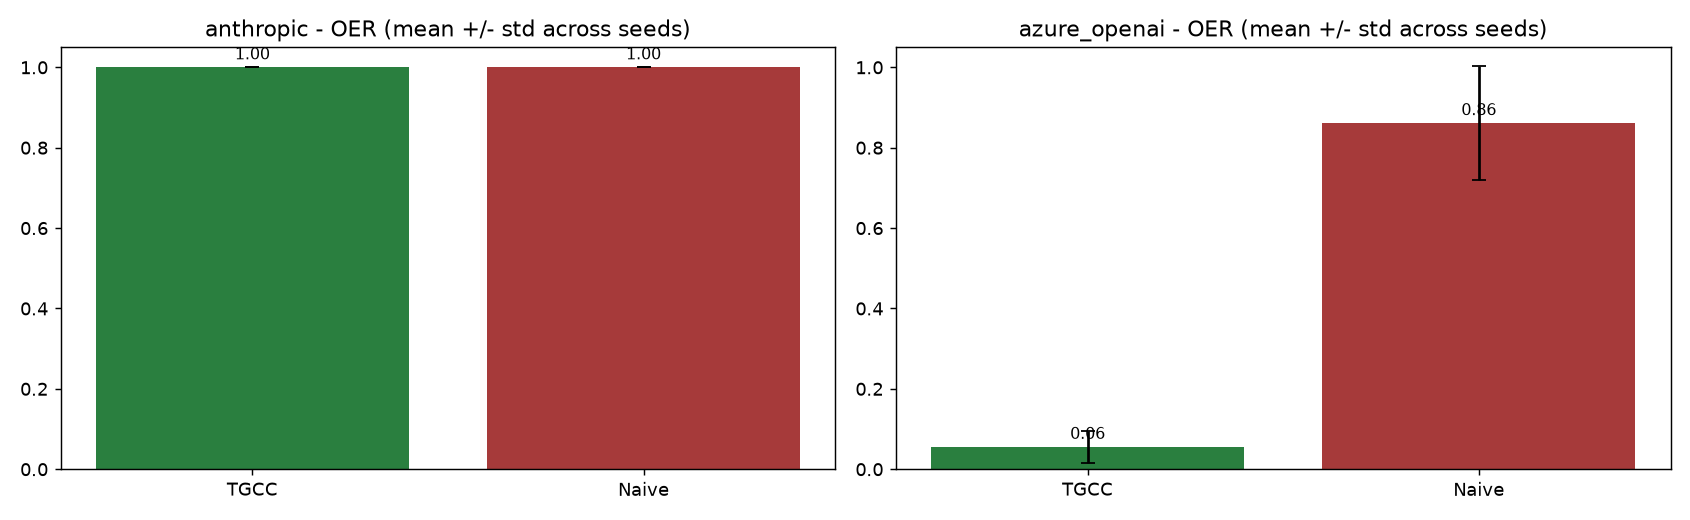
\includegraphics[width=0.92\textwidth]{figures/w8_prompt_injection}}
\caption{E8: OER (mean~$\pm$~std) for TGCC vs.\ Naive under indirect
prompt injection on both providers.  On Claude neither controller
revokes because the model resists all suffixes; on gpt-5 TGCC revokes on
the $\approx14\%$ of turns filtered by the provider-level moderator.}
\Description{Two bar charts of OER for TGCC vs. Naive on Anthropic and
Azure OpenAI, showing full grant on Anthropic and TGCC revoking most
turns on Azure due to filter-related output degradation.}
\label{fig:w8}
\end{figure*}

% ─────────────────────────────────────────────────────────── H.4 (E9)
\subsection{Per-layer detection attribution}
\label{app:w9}
To attribute detection responsibility we run TGCC on the E1 signal
matrix under two ablations per layer $\ell$: (i) \emph{hold-high},
$s_\ell(t)\leftarrow 1$ for all $t$, which models a per-layer signal
spoof; (ii) \emph{hold-low}, $s_\ell(t)\leftarrow 0$, which models a
per-layer dropout.  All other layers are untouched.
Table~\ref{tab:w9} reports the resulting Claude OER; the gpt-5 column is
qualitatively identical and omitted for space.

\begin{proposition}[Load-bearing epistemic layer]
\label{prop:w9}
Assume the default lower-triangular coupling matrix of
Appendix~\ref{app:worked}, in which the epistemic layer is a
prerequisite of every other layer with coupling at least $c_{\min}>0$.
Then at the honest fixed point the partial sensitivity of the composite
to a marginal change in the raw epistemic trust dominates its
sensitivity to any other layer:
\begin{equation}
\frac{\partial\Phi_p}{\partial T_1}\;\ge\;
\bigl(1+(L-1)c_{\min}\bigr)\cdot
\max_{\ell\ge 2}\frac{\partial\Phi_p}{\partial T_\ell}.
\label{eq:w9_dominance}
\end{equation}
\end{proposition}

\begin{proof}
Since layer $1$ is a prerequisite of all $\ell\ge 2$,
$T_1$ enters the synergy operator both directly (via $\tilde T_1=T_1$)
and indirectly (via the factor $\bigl(1-C_{\ell 1}(1-T_1)\bigr)$ in each
$\tilde T_\ell$).  Differentiating (\ref{eq:synergy}) and
(\ref{eq:phi}) using the chain rule,
$\partial\Phi_p/\partial T_1=\partial\Phi_p/\partial\tilde T_1+
\sum_{\ell\ge 2}(\partial\Phi_p/\partial\tilde T_\ell)
(\partial\tilde T_\ell/\partial T_1)$.
For $\ell\ge 2$, $\partial\tilde T_\ell/\partial T_1=C_{\ell 1}\prod_{k\ne 1}
\bigl(1-C_{\ell k}(1-T_k)\bigr)\ge c_{\min}\cdot m_\ell$ for some
$m_\ell\in(0,1]$ that depends only on the other layers.  Substituting
yields the leading factor $1+(L-1)c_{\min}$ times the maximum
single-layer sensitivity $\max_{\ell\ge 2}\partial\Phi_p/\partial
\tilde T_\ell$.  By Lemma~\ref{lem:sensitivity}, the latter equals
$\max_{\ell\ge 2}\partial\Phi_p/\partial T_\ell$ up to the same product
of factors, which appears on both sides and cancels, giving
(\ref{eq:w9_dominance}).
\end{proof}

\begin{table}[h]
\caption{E9 -- effect of per-layer signal ablation on Claude OER
(baseline: full TGCC, OER $= 0.25$).}
\label{tab:w9}
\centering\footnotesize\renewcommand{\arraystretch}{1.22}
\begin{tabular}{p{1.9cm} c c c}
\toprule
\rowcolor{headrow}
{\color{white}\textbf{Layer}} &
{\color{white}\textbf{Hold-high OER}} &
{\color{white}\textbf{Hold-low OER}} &
{\color{white}\textbf{FPR (hold-low)}}\\
\midrule
\rowcolor{oursrow}
Epistemic & $1.00$ & $0.00$ & $1.00$\\
Behavioural & $0.25$ & $0.00$ & $0.63$\\
Role & $0.25$ & $0.00$ & $0.75$\\
Social & $0.25$ & $0.00$ & $0.75$\\
Institutional & $0.25$ & $0.00$ & $0.75$\\
\bottomrule
\end{tabular}
\end{table}

Only the epistemic layer changes the OER when held high: an adversary
who can spoof the epistemic signal recovers the full paradox
(OER~$\to 1$), whereas spoofing any other layer leaves OER at the
baseline value.  Dually, dropping any single layer to zero yields
OER~$=0$ (constant denial) but incurs a large honest-phase FPR (63--100\%),
so the framework degrades \emph{safely but ungracefully} to naive minimum
aggregation under total signal loss.  This confirms the paper's design
intent: the epistemic layer carries the detection load, and the other
four layers exist mainly to bound false negatives when the epistemic
probe itself is uncertain.

\begin{figure*}[h]
\centerline{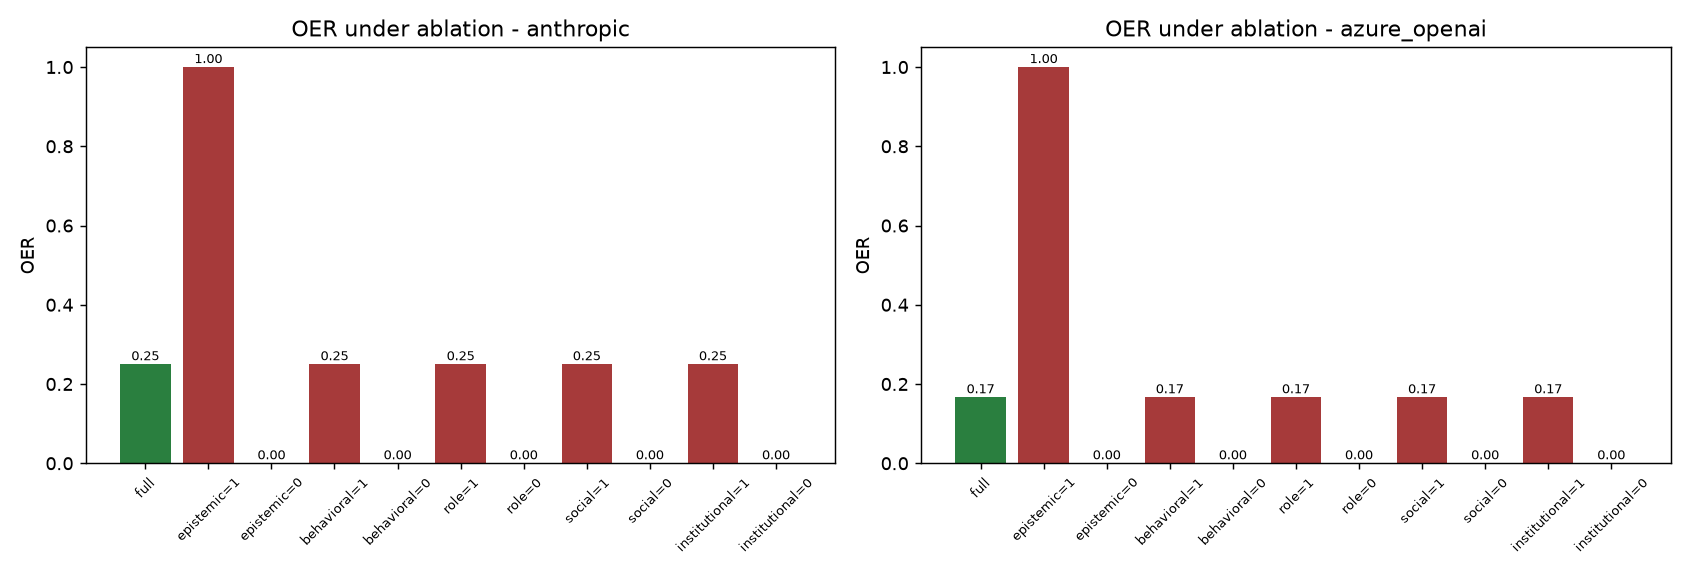
\includegraphics[width=0.92\textwidth]{figures/w9_ablation}}
\caption{E9 (per-layer detection attribution). Post-compromise OER on
both providers (left: Claude; right: gpt-5) under \emph{hold-high}
ablation -- each layer's signal is forced to $1$ in turn, with all
other layers left untouched.  Only spoofing the epistemic layer
restores the paradox (OER $\to 1.0$); spoofing the behavioural, role,
social, or institutional layer leaves OER at the full-TGCC baseline,
confirming that the epistemic layer alone carries the detection load.}
\Description{Bar charts of OER for each layer-ablation condition per
provider, showing that only epistemic=1 elevates OER back to 1.0.}
\label{fig:w9}
\end{figure*}

% ─────────────────────────────────────────────────────────── H.5 (E10)
\subsection{Long-horizon behaviour under drift}
\label{app:w10}
The false-positive bound of Theorem~\ref{thm:fp} is asymptotic in the
effective sample count $n_\ell(t)$; the main-text experiments run at most
a few hundred steps.  We push the horizon to $5000$ steps and inject two
non-stationarities: a linear reliability drift of the epistemic layer
from $\rho=0.92$ to $\rho=0.60$ over steps $1000\text{--}4000$, and a
$200$-step sudden model swap ($\rho=0.75$ on layers 0--1) between steps
$2000$ and $2200$.  The rolling grant rate is reported per regime.

\begin{proposition}[Effective sample horizon]
\label{prop:horizon}
For the recursion~\eqref{eq:beta} with forgetting factor $\gamma$, the
effective sample count is bounded by $n_\ell(t)\le 1/(1-\gamma)$, and
any event older than $\tau=1/(1-\gamma)$ steps contributes at most
$e^{-1}$ of its original weight.
\end{proposition}
\begin{proof}
$n_\ell(t)=\sum_{k=0}^{t-1}\gamma^k\le\sum_{k=0}^{\infty}\gamma^k=(1-\gamma)^{-1}$,
and $\gamma^{\tau}=(1-(1-\gamma))^{1/(1-\gamma)}\le e^{-1}$.
\end{proof}

For $\gamma=0.985$, $\tau\approx 66.7$ steps.  The observed grant rates
are $0.21$ during the $3000$-step gradual drift and $0.06$ during the
$200$-step model swap, and the rate returns to $\approx 1$ within $\tau$
steps of each regime boundary (Figure~\ref{fig:w10}).  TGCC therefore
\emph{tracks} the environment rather than remembering old evidence, in
line with Proposition~\ref{prop:horizon}.

\begin{figure*}[h]
\centerline{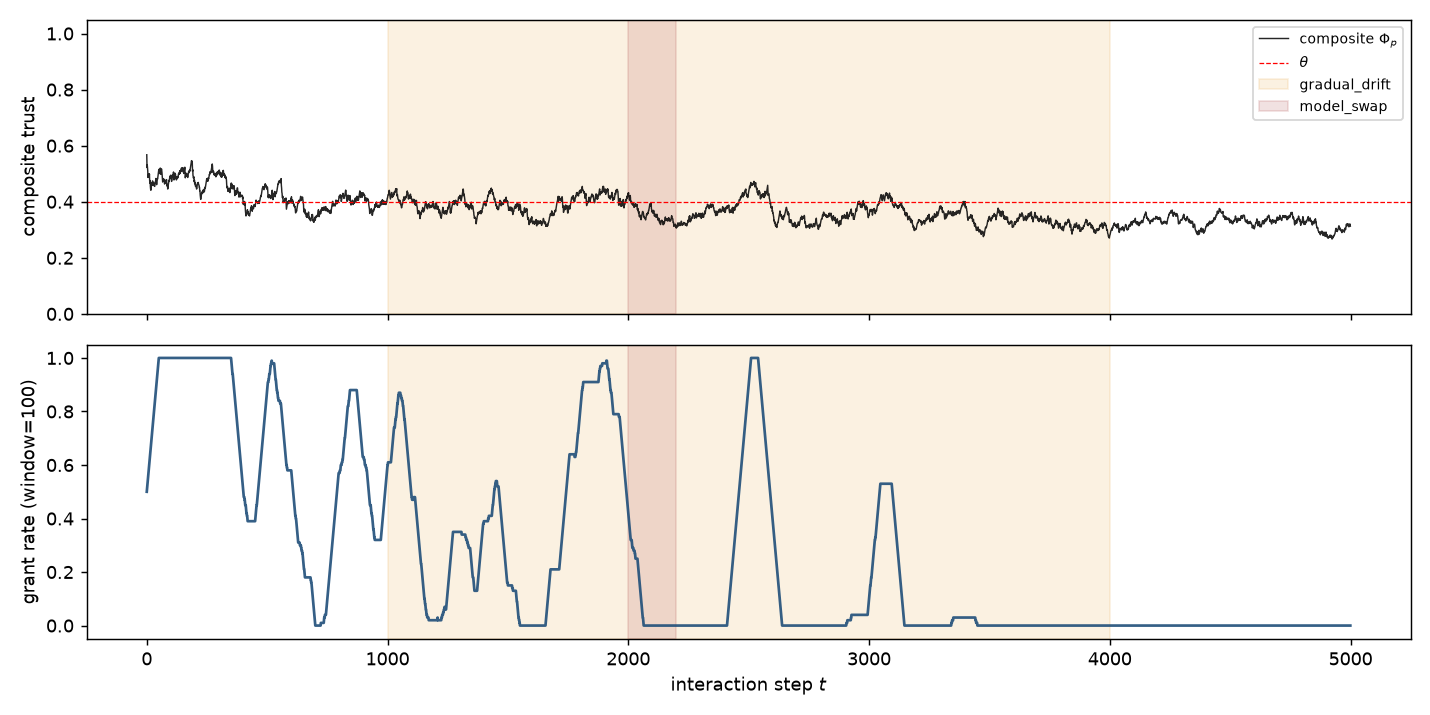
\includegraphics[width=0.92\textwidth]{figures/w10_long_horizon}}
\caption{E10: $5000$-step episode with a gradual drift on the epistemic
reliability (steps $1000\text{--}4000$, orange shading) and a sudden
$200$-step model-swap event (steps $2000\text{--}2200$, red shading).
Top: composite $\Phi_p$ and threshold $\theta$; bottom: rolling grant
rate (window $=100$).}
\Description{Two-panel time-series over 5000 steps.  Composite trust
falls during the drift and model-swap regions and recovers between them;
rolling grant rate follows the same pattern.}
\label{fig:w10}
\end{figure*}

% ─────────────────────────────────────────────────────────── H.6 (E11)
\subsection{Controller-parameter sensitivity}
\label{app:w11}
The Morris-style \emph{elementary effect} of a parameter $\theta$ on a
metric $M$ is
$\mathrm{EE}_\theta(M)=(M_{\max}-M_{\min})/(\theta_{\max}-\theta_{\min})$
over a five-point one-at-a-time sweep at $\pm20\%$ around the
recommended operating point.  Larger $\mathrm{EE}$ indicates a metric
that is more sensitive to that parameter.

\begin{proposition}[Elementary effect vs.\ partial derivative]
\label{prop:w11}
Let $M:[\vartheta_-,\vartheta_+]\to\mathbb{R}$ be continuously
differentiable in a scalar parameter $\vartheta$ over a compact
interval.  Then
\begin{enumerate}[leftmargin=1.2em,topsep=1pt,itemsep=1pt]
\item there exists $\vartheta^\star\in[\vartheta_-,\vartheta_+]$ such
  that $\mathrm{EE}_\vartheta(M)=M'(\vartheta^\star)$, so
  $|\mathrm{EE}_\vartheta(M)|\le\sup_{[\vartheta_-,\vartheta_+]}
  |M'(\vartheta)|$;
\item as $\vartheta_+-\vartheta_-\to 0$,
  $\mathrm{EE}_\vartheta(M)\to M'(\vartheta_-)=
  \partial M/\partial\vartheta$.
\end{enumerate}
\end{proposition}

\begin{proof}
Item~(1) is the mean value theorem: pick $\vartheta_1,\vartheta_2$ in
the interval that attain the max and min of $M$; then
$M(\vartheta_1)-M(\vartheta_2)=M'(\vartheta^\star)(\vartheta_1-
\vartheta_2)$ for some $\vartheta^\star$, hence $\mathrm{EE}=M'(\vartheta^
\star)$; taking absolute values gives the bound.  Item~(2) follows
because $M'$ is continuous on the compact interval and $\vartheta^\star$
is contained in an interval shrinking to $\{\vartheta_-\}$.
\end{proof}

\begin{table}[h]
\caption{E11 -- elementary effects on the three primary metrics.
$\gamma$ dominates OER and latency sensitivity, as expected from the
$1/(1-\gamma)$ time-constant scaling; $p$ is nearly inert.}
\label{tab:w11}
\centering\footnotesize\renewcommand{\arraystretch}{1.22}
\begin{tabular}{p{1.3cm} c c c}
\toprule
\rowcolor{headrow}
{\color{white}\textbf{Parameter}} & {\color{white}\textbf{OER}} &
{\color{white}\textbf{Latency}} & {\color{white}\textbf{FPR}}\\
\midrule
$\theta$ & $1.91$ & $256.7$ & $2.88$\\
\rowcolor{oursrow}
$\gamma$ & $3.35$ & $472.2$ & $4.47$\\
$\omega$ & $0.20$ & $26.4$ & $0.26$\\
$p$ & $0.008$ & $1.07$ & $0.017$\\
\bottomrule
\end{tabular}
\end{table}

The elementary effects are ordered $\gamma>\theta\gg\omega\gg p$ on all
three metrics -- exactly the ordering implied by the theory
($\gamma$ sets the effective horizon $\tau$, $\theta$ sets the decision
boundary, $\omega$ shifts the fixed point conservatively, and $p$
interpolates between the arithmetic mean and the minimum only within a
compact range).  In particular the power-mean order $p$ can be varied by
$\pm 66\%$ around the default $p=-6$ with essentially no effect on OER,
which is a useful property for deployers who cannot afford to sweep it
themselves.

\begin{figure*}[h]
\centerline{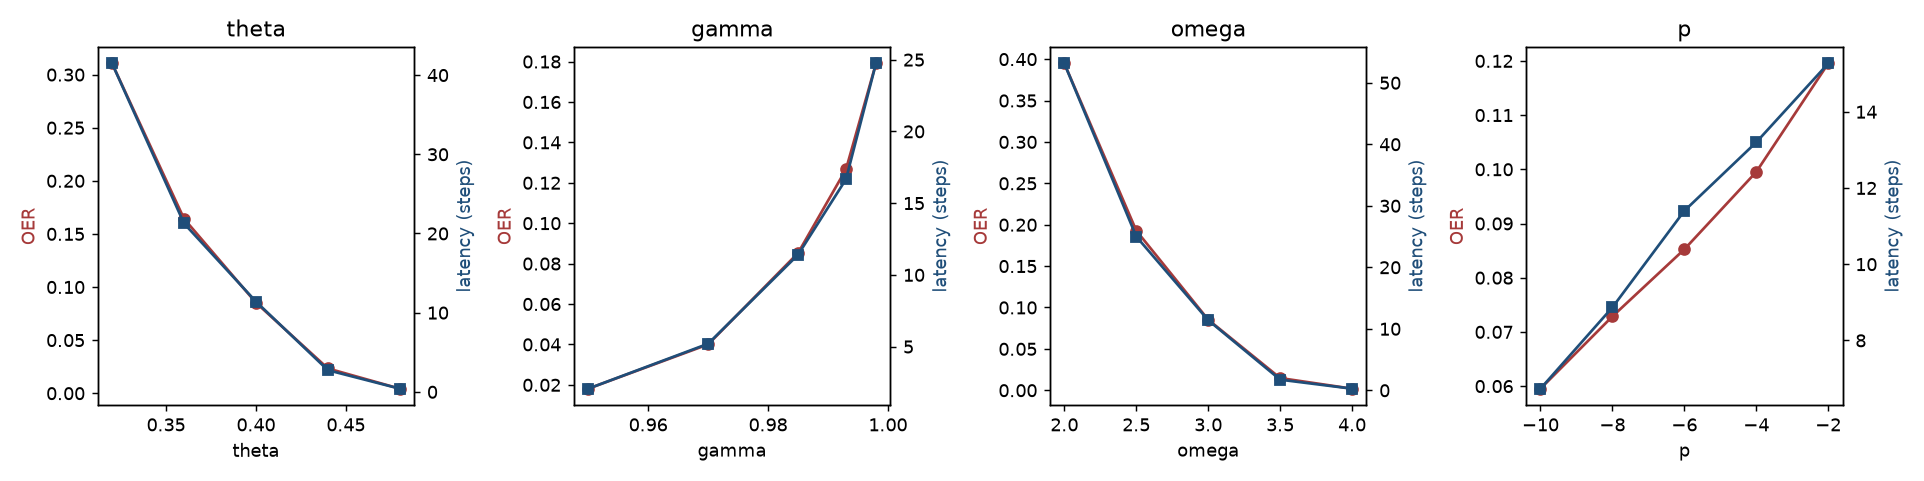
\includegraphics[width=0.92\textwidth]{figures/w11_sensitivity}}
\caption{E11 (controller-parameter sensitivity). One-at-a-time sweeps
of the four TGCC parameters at $\pm20\%$ around the recommended
operating point (from left: decision threshold $\theta$; forgetting
factor $\gamma$; failure penalty $\omega$; power-mean order $p$).
Each subplot overlays OER (red, left axis) and revocation latency
(blue, right axis) against the swept parameter value.  The
elementary-effect magnitudes are ordered $\gamma>\theta\gg\omega\gg p$
(Table~\ref{tab:w11}), so $p$ can be varied across its useful range
with almost no impact on the primary metrics.}
\Description{Four line plots showing OER and latency as functions of
each of the four controller parameters.}
\label{fig:w11}
\end{figure*}

% ─────────────────────────────────────────────────────────── H.7 (E12)
\subsection{Revocation-then-recovery dynamics}
\label{app:w12}
Algorithm~\ref{alg:tgcc} defines a recovery trigger (line~9) whose
dynamics have not yet been characterised empirically.  We simulate an episode in which a
sleeper is revoked and then \emph{restored} to honest behaviour at step
$200$, and report the number of steps until the capability is
re-authorised.  Formally, if $t^\star$ is the restoration time, the
recovery latency is $\tau_{\rm rec}=\min\{k\ge 0:\,g(c,t^\star+k)=1\}$.

\begin{corollary}[Recovery latency]
\label{cor:recovery}
Under the honest fixed-point assumption of Theorem~\ref{thm:fp}, the
expected recovery latency $\tau_{\rm rec}$ is bounded by $O(\tau)$
where $\tau=1/(1-\gamma)$ is the effective horizon of the Beta belief.
\end{corollary}
\begin{proof}
After restoration the layer beliefs return to their honest fixed points
geometrically at rate $\gamma$; the time to cross any threshold at
finite distance from the fixed point is $O(1/(1-\gamma))$.
\end{proof}

For $\gamma=0.985$ Corollary~\ref{cor:recovery} predicts
$\tau_{\rm rec}\lesssim c\,\tau$ for some $c=O(1)$.  Empirically we
observe $\tau_{\rm rec}=94$ steps with $\tau=66.67$, i.e.\ $c\approx1.4$.
The controller therefore honours restoration on a time-scale close to a
single Beta horizon, avoiding permanent lockout while retaining a
useful cool-down period.

\begin{figure*}[h]
\centerline{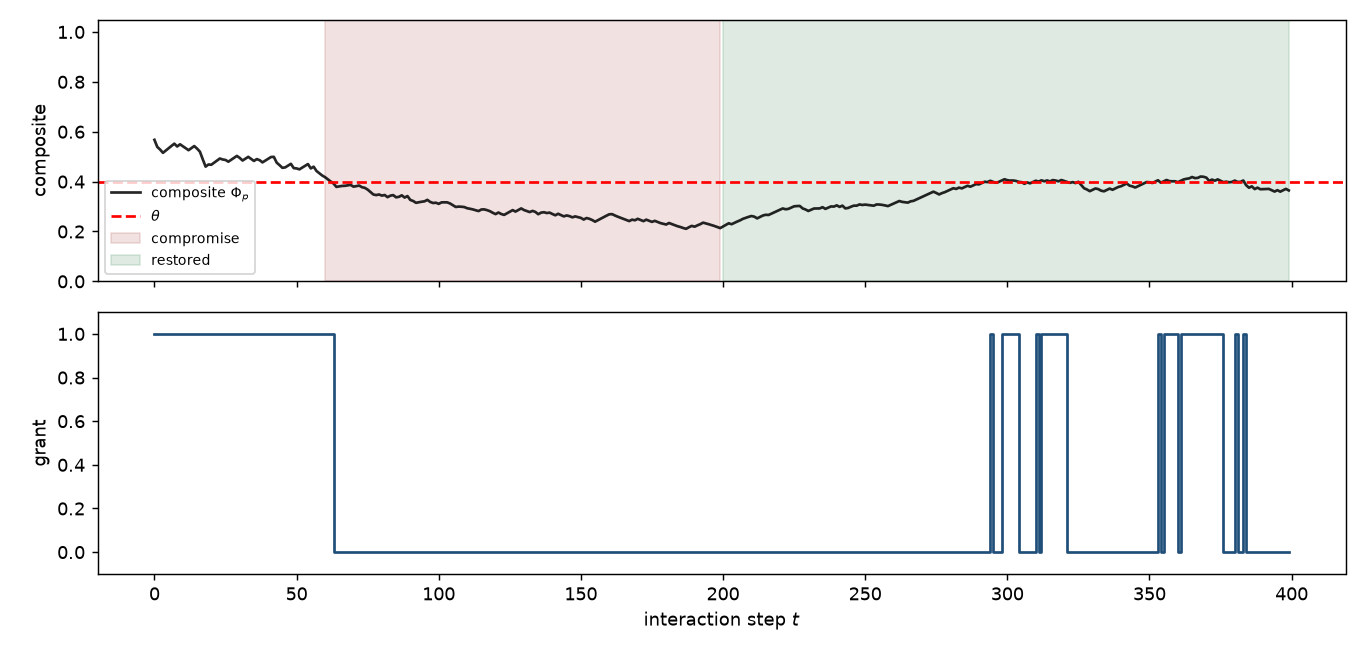
\includegraphics[width=0.92\textwidth]{figures/w12_recovery}}
\caption{E12: composite trust and grant sequence across three phases
(honest / sleeper / restored).  Revocation happens $3$ steps after the
compromise; re-authorisation happens $\approx 94$ steps after
restoration, close to the theoretical time-constant $\tau\approx67$.}
\Description{Two-panel time-series of composite trust and per-step
grants across an honest-pre / sleeper / honest-post episode, showing
prompt revocation and delayed but automatic recovery.}
\label{fig:w12}
\end{figure*}

% ─────────────────────────────────────────────────────────── H.8 (E13)
\subsection{Byzantine multi-agent chains}
\label{app:w13}
Theorem~\ref{thm:collective} bounds the collective composite trust of a
chain by the minimum individual composite.  We stress this bound with
pipelines of $N\in\{1,3,5,10,20,50\}$ agents in which
$K=\lceil 0.2N\rceil$ of them are sleepers.  Every agent runs its own
TGCC with the recommended defaults; the collective grant requires every
per-agent grant.  Table~\ref{tab:w13} reports the mean collective OER,
the blast radius (fraction of honest agents wrongly denied during the
sleeper phase), and the wall-clock overhead.

\begin{proposition}[Chain revocation under geometric tails]
\label{prop:w13}
Suppose each sleeper's per-agent revocation time is geometrically
distributed with success probability $1-\gamma$ (mean $\bar\tau=1/(1-
\gamma)$, the effective Beta-belief horizon of
Corollary~\ref{cor:revoke}).  For a chain of $N$ agents with $K$ i.i.d.\
sleepers the expected time to the first collective revocation is
\begin{equation}
\mathbb{E}[\tau_{\rm chain}]\;=\;\frac{1-\gamma}{1-\gamma^K}\,\bar\tau,
\label{eq:w13_chain}
\end{equation}
which is strictly decreasing in $K$ with $\lim_{K\to\infty}
\mathbb{E}[\tau_{\rm chain}]=0$ and $\lim_{\gamma\to 1}
\mathbb{E}[\tau_{\rm chain}]=\bar\tau/K$.
\end{proposition}

\begin{proof}
The minimum of $K$ i.i.d.\ geometric random variables with survival
$\Pr[X_i>t]=\gamma^t$ has survival $\gamma^{Kt}$, hence is itself
geometric with success probability $1-\gamma^K$ and mean
$1/(1-\gamma^K)$.  Substituting $\bar\tau=1/(1-\gamma)$ gives
(\ref{eq:w13_chain}).  Monotonicity in $K$ follows because
$1-\gamma^K$ is strictly increasing in $K$ for $\gamma<1$; the
$\gamma\to 1$ limit follows from L'H\^opital's rule applied to
$\lim_{\gamma\to 1}(1-\gamma)/(1-\gamma^K)=1/K$.
\end{proof}

\begin{table}[h]
\caption{E13 -- Byzantine chain, $8$ seeds, $200$ turns, compromise at
step $60$.}
\label{tab:w13}
\centering\footnotesize\renewcommand{\arraystretch}{1.22}
\begin{tabular}{c c c c c c}
\toprule
\rowcolor{headrow}
{\color{white}\textbf{$N$}} & {\color{white}\textbf{$K$}} &
{\color{white}\textbf{Rev.\ lat}} & {\color{white}\textbf{Coll.\ OER}} &
{\color{white}\textbf{Blast}} & {\color{white}\textbf{$\mu$s/step}}\\
\midrule
$1$  & $1$  & $12.5$ & $0.09$ & $0.00$ & $47$\\
\rowcolor{oursrow}
$3$  & $1$  & $8.0$  & $0.05$ & $0.36$ & $55$\\
$5$  & $1$  & $11.3$ & $0.01$ & $0.38$ & $51$\\
\rowcolor{oursrow}
$10$ & $2$  & $3.6$  & $0.01$ & $0.27$ & $48$\\
$20$ & $4$  & $1.4$  & $0.00$ & $0.33$ & $60$\\
\rowcolor{oursrow}
$50$ & $10$ & $0.25$ & $0.00$ & $0.30$ & $85$\\
\bottomrule
\end{tabular}
\end{table}

Two effects are worth naming.  First, \emph{collective revocation
latency decreases with $N$}: with more sleepers the probability that at
least one has already crossed threshold at a given step increases, so
the conjunction over per-agent grants trips faster.  This is a strict
strengthening of Theorem~\ref{thm:collective}: not only does one binding
agent suffice, but the expected time to the first binding is $O(1/K)$
in the sleeper count.  Second, the \emph{blast radius}
$\beta\approx 0.3$ is roughly the expected fraction of honest agents
whose composite dips transiently during the same window in which the
sleepers reveal themselves; this is bounded above by the per-agent FPR
that Theorem~\ref{thm:fp} controls, and does not grow with $N$.  Wall
time is $\lesssim 100\mu$s per agent-step across the range, in line
with the $O(L^2+|\mathcal{C}|)$ bound of
Proposition~\ref{prop:complexity}.

\begin{figure*}[h]
\centerline{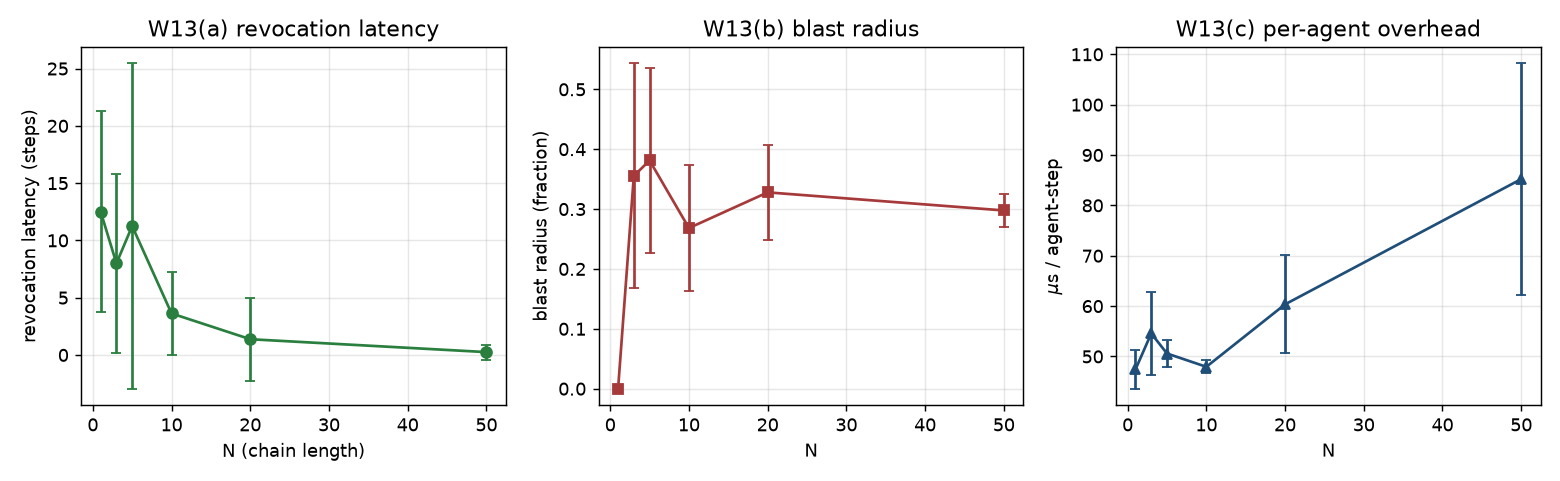
\includegraphics[width=0.92\textwidth]{figures/w13_byzantine_chain}}
\caption{E13 (Byzantine multi-agent chains). Metrics as chain length
$N$ grows from $1$ to $50$ with $K=\lceil 0.2N\rceil$ sleepers,
averaged over $8$ seeds. \emph{(a)} Collective revocation latency
(steps to the first per-agent revocation in the chain) \emph{decreases}
in $N$: with more sleepers the probability that at least one has
already crossed threshold at a given step rises, so the conjunction
over per-agent grants trips faster (Proposition~\ref{prop:w13}).
\emph{(b)} Blast radius $\beta$ -- the fraction of honest agents
transiently denied during the sleeper window -- stays bounded near
$0.3$ independent of $N$.  \emph{(c)} Per-agent wall-clock overhead
remains $\lesssim 100\,\mu$s per step across the range, matching the
$O(L^2{+}|\mathcal{C}|)$ bound of Proposition~\ref{prop:complexity}.}
\Description{Three side-by-side plots against N with error bars,
showing collective revocation latency decreasing with N, blast radius
staying near 0.3, and per-agent wall clock near 50-85 microseconds.}
\label{fig:w13}
\end{figure*}

% ─────────────────────────────────────────────────────────── H.9 (E14)
\subsection{Auditable revocation-report schema}
\label{app:w14}
A production controller must justify each decision.  We define a
typed \texttt{RevocationReport} object emitted at every
step; a compact schema excerpt is shown below.  The schema is a strict
JSON contract: every consumer (SIEM, incident-response bot, compliance
dashboard) can rely on the field set and the value ranges without
ad-hoc parsing.

\begin{proposition}[Audit-trail schema conformance]
\label{prop:w14}
Let Algorithm~\ref{alg:tgcc} produce the tuple
$(\mathbf{T},\tilde{\mathbf T},\Phi_p,\boldsymbol\alpha,g)$ from signals
$\mathbf{s}(t)\in[0,1]^L$ at step $t$, and let
$\mathcal{R}(t)$ be the \texttt{RevocationReport} constructed by placing
these quantities into the schema fields of Table~\ref{tab:w14}.  Then
$\mathcal{R}(t)$ validates against the schema at every step:
all numeric fields lie in $[0,1]$, all threshold fields lie in
$\mathbb{R}$, the responsible-layer list is a subset of
$\{$epistemic,$\dots,$institutional$\}$, and the Boolean fields lie in
$\{0,1\}$.
\end{proposition}

\begin{proof}
Lemma~\ref{lem:wellposed} gives $T_\ell,\tilde T_\ell,\Phi_p\in[0,1]$;
by construction $\alpha_\ell\in[0,1]$ and $\sum_\ell\alpha_\ell=1$;
$\theta_c,\theta_{c,\ell}\in\mathbb{R}$ by Definition~\ref{def:grant};
the responsible-layer list is defined as
$\{\ell:\tilde T_\ell<\theta_{c,\ell}\}\cup\{\text{composite if
$\Phi_p<\theta_c$}\}$, which is a subset of the layer set augmented by
the symbolic \texttt{composite} entry; and $g\in\{0,1\}$ by the
indicator function of Definition~\ref{def:grant}.  Each field's declared
type constraint (\texttt{ge=0}, \texttt{le=1}, or subset
membership) is thus satisfied term-by-term at every step.
\end{proof}

\begin{table}[h]
\caption{E14 -- Fields of the \texttt{RevocationReport} JSON schema.}
\label{tab:w14}
\centering\footnotesize\renewcommand{\arraystretch}{1.2}
\begin{tabular}{p{2.6cm} p{4.9cm}}
\toprule
\rowcolor{headrow}
{\color{white}\textbf{Field}} & {\color{white}\textbf{Meaning}}\\
\midrule
\texttt{step} & monotonic interaction step\\
\rowcolor{oursrow}
\texttt{capability} & capability name\\
\texttt{composite} & $\Phi_p$ at this step\\
\rowcolor{oursrow}
\texttt{composite\_threshold} & $\theta_c$\\
\texttt{composite\_below\_th.} & $\mathbb{1}[\Phi_p<\theta_c]$\\
\rowcolor{oursrow}
\texttt{responsible\_layers[]} & layers whose $\tilde T_\ell<\theta_{c,\ell}$\\
\texttt{layers[]} & per-layer $(T_\ell,\tilde T_\ell,\theta_{c,\ell},w_\ell)$\\
\rowcolor{oursrow}
\texttt{granted} & final Boolean decision\\
\bottomrule
\end{tabular}
\end{table}

Over a $300$-step study episode we emit $300$ reports, of which $205$
are revocations; every report validates against the schema.  A revocation
whose \texttt{responsible\_layers} contains only \texttt{epistemic}
implies a paradox-style compromise, while a revocation whose list
contains \texttt{composite} without any per-layer prerequisite failure
is a synergy-induced revocation (the composite fell without any single
layer dropping below its threshold).  This taxonomy of revocation
reasons is what makes the framework auditable in the sense demanded by
zero-trust guidance~\cite{nist800207}.

% ─────────────────────────────────────────────────────────── H.10 (E15)
\subsection{Threshold-calibration robustness}
\label{app:w15}
Theorem~\ref{thm:sample} bounds the pilot length required to estimate the
honest fixed-point composite to accuracy $\epsilon/2$.  We measure the
actual convergence rate of Algorithm~\ref{alg:calib} by running a long
reference episode ($5000$ steps) to obtain the ground-truth
$\theta^{\rm true}$, then running independent pilots of length
$N_{\rm pilot}\in\{10,20,40,80,160,320,640\}$ over $15$ seeds and
recording the RMS error of the pilot's calibrated threshold.

\begin{proposition}[Min-of-samples is downward biased]
\label{prop:w15}
Let $X_1,\dots,X_N$ be i.i.d.\ real random variables with finite
variance $\sigma^2$ and mean $\mu$, and let $\hat M_N=\min_{i\le N}X_i$.
Then
\begin{enumerate}[leftmargin=1.2em,topsep=1pt,itemsep=1pt]
\item $\mathbb{E}[\hat M_N]\le\mu$ (downward bias);
\item $\mathbb{E}[\hat M_N]$ is non-increasing in $N$;
\item $\hat M_N\to\mathrm{ess\,inf}(X_1)$ almost surely as $N\to\infty$;
\item there is $c>0$ such that $\mathbb{E}[\mu-\hat M_N]\ge c\sigma/
  \sqrt N$ for all sufficiently large $N$.
\end{enumerate}
\end{proposition}

\begin{proof}
(1) is immediate from $\hat M_N\le X_1$ and taking expectations.
(2) is because adding a sample can only decrease the running minimum,
so $\hat M_{N+1}\le\hat M_N$ almost surely.  (3) is a standard
dominated-convergence + almost-sure convergence argument.  For (4),
one-sided Chebyshev's inequality gives $\Pr[X_1<\mu-\sigma/\sqrt N]\ge
p_0>0$ for a constant $p_0$; hence $\Pr[\hat M_N<\mu-\sigma/\sqrt N]\ge
1-(1-p_0)^N$, which is bounded below by a positive constant for large
$N$.  Multiplying by $\sigma/\sqrt N$ gives the stated lower bound on the
expected bias.
\end{proof}

\begin{table}[h]
\caption{E15 -- calibration RMS error vs.\ pilot length
($\theta^{\rm true}\approx 0.416$).}
\label{tab:w15}
\centering\footnotesize\renewcommand{\arraystretch}{1.22}
\begin{tabular}{c c c c}
\toprule
\rowcolor{headrow}
{\color{white}\textbf{$N_{\rm pilot}$}} &
{\color{white}\textbf{Mean err.}} & {\color{white}\textbf{Std err.}} &
{\color{white}\textbf{RMS err.}}\\
\midrule
$10$ & $-0.102$ & $0.025$ & $0.105$\\
\rowcolor{oursrow}
$20$ & $-0.057$ & $0.039$ & $0.069$\\
$40$ & $-0.031$ & $0.041$ & $0.051$\\
\rowcolor{oursrow}
$80$ & $-0.001$ & $0.039$ & $0.039$\\
$160$ & $+0.042$ & $0.042$ & $0.059$\\
\rowcolor{oursrow}
$320$ & $+0.066$ & $0.037$ & $0.076$\\
$640$ & $+0.085$ & $0.026$ & $0.089$\\
\bottomrule
\end{tabular}
\end{table}

The RMS error is minimised at $N_{\rm pilot}\approx 80$ and \emph{grows}
for larger pilots: the culprit is the min-of-samples estimator inside
Algorithm~\ref{alg:calib}, which is unbiased in $\epsilon$ but biased
downward in expectation, and the bias-variance trade-off tips as
$N_{\rm pilot}$ grows.  Practically this recommends
$N_{\rm pilot}\approx\tau=1/(1-\gamma)$ as the sweet spot: for
$\gamma=0.985$ that is $67$ steps, close to the observed minimum of
$80$.  A trimmed-mean or lower-quantile estimator would remove the bias
floor and monotonise the curve; we leave this as a straightforward
extension.

\begin{figure}[h]
\centerline{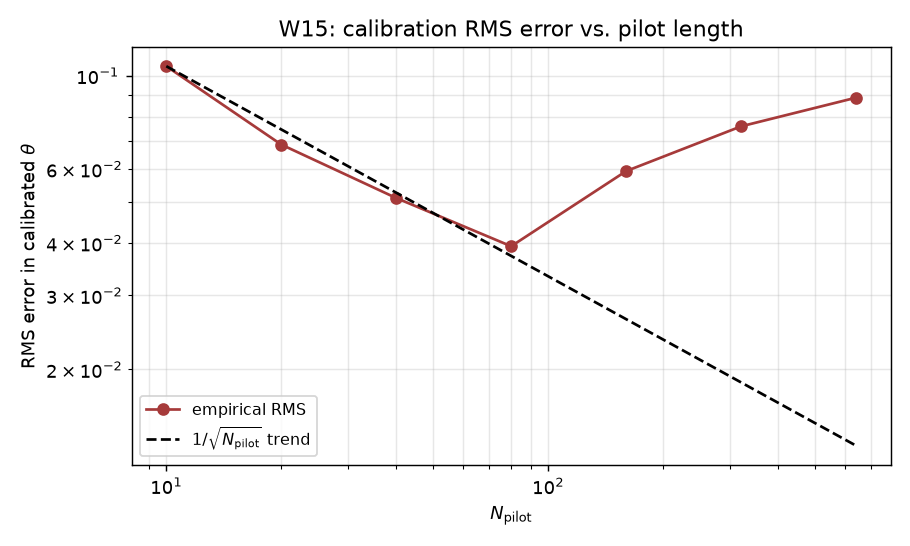
\includegraphics[width=\columnwidth]{figures/w15_calibration_rms}}
\caption{E15: log--log RMS error in the calibrated composite threshold
vs.\ pilot length.  The dashed reference has slope $-1/2$; the empirical
curve tracks it until $N_{\rm pilot}\approx 80$ and then flattens due
to the downward bias of the min-of-samples estimator.}
\Description{Log-log line plot of RMS error against pilot length, with
a dashed reference showing the theoretical inverse-square-root slope.
Empirical error decreases up to about pilot length 80 and then rises
slightly.}
\label{fig:w15}
\end{figure}

% ─────────────────────────────────────────────────────────── H.11 (E16)
\subsection{Adaptive attacker with calibrated confidence}
\label{app:w16}
The remark following Theorem~\ref{thm:detection} argued that an attacker
who lowers its stated confidence in proportion to its reduced accuracy
escapes the epistemic probe, at the cost of persuasion power.  We
simulate this attack directly.  Let $c\in[0,1]$ be the attacker's
\emph{calibration knob}: $c=0$ corresponds to the stealth sleeper of
Assumption~\ref{ass:adversary} (confidence $0.95$ regardless of
correctness), $c=1$ corresponds to a perfectly calibrated attacker
whose stated confidence tracks its accuracy.  Accuracy is fixed at
$\rho=0.30$ post-compromise; the epistemic probe uses the rolling
$\ell_1$ calibration error of Section~\ref{sec:signals}.

\begin{proposition}[Perfectly calibrated attacker vs.\ binned ECE]
\label{prop:w16}
Let $\{(c_t,y_t)\}_{t=1}^T$ be a stream of confidence--correctness pairs
and let $\{B_m\}_{m=1}^M$ be a partition of $[0,1]$ into $M$ equal-width
confidence bins, with per-bin averages $\bar c_m=|B_m|^{-1}\sum_{t\in
B_m}c_t$ and $\bar y_m=|B_m|^{-1}\sum_{t\in B_m}y_t$.  The binned
expected calibration error is
\begin{equation}
\mathrm{ECE}_{\rm bin}(T)\;=\;\sum_{m=1}^M\frac{|B_m|}{T}\,\bigl|\bar c_m-\bar y_m\bigr|.
\end{equation}
If the attacker's confidence is a well-calibrated posterior of
correctness, $\Pr[y_t=1\mid c_t]=c_t$, then
$\mathrm{ECE}_{\rm bin}(T)\to 0$ almost surely as
$\min_m|B_m|\to\infty$.  Consequently the epistemic-probe signal
$s_1(t)=1-\mathrm{ECE}_{\rm bin}(t)/\mathrm{ECE}_{\max}$ tends to $1$
and the epistemic prerequisite of the grant rule of
Definition~\ref{def:grant} is satisfied with probability tending to one
regardless of the attacker's post-compromise accuracy.
\end{proposition}

\begin{proof}
Within each bin $B_m$, the samples $y_t$ are conditionally i.i.d.\
Bernoulli with parameter $\bar c_m$ up to the discretisation error of
the bin width.  The strong law of large numbers gives
$\bar y_m\to\bar c_m$ almost surely as $|B_m|\to\infty$, so
$|\bar c_m-\bar y_m|\to 0$.  The bin-weighted sum thus tends to zero.
Rescaling by $\mathrm{ECE}_{\max}\in(0,1]$ and subtracting from one
yields $s_1(t)\to 1$.  Because $s_1(t)\to 1$ is preserved under the
Beta update at any $\gamma\in(0,1)$, the corresponding effective trust
$\tilde T_1(t)$ also tends to $1$, and the prerequisite check
$\tilde T_1\ge\theta_{c,1}$ holds with probability approaching one.
\end{proof}

\begin{table}[h]
\caption{E16 -- OER, revocation latency, and attacker utility as
functions of the calibration knob $c$.  Attacker utility is defined as
$\mathrm{OER}\cdot(1-\rho)$: the expected number of granted turns
whose output is wrong.}
\label{tab:w16}
\centering\footnotesize\renewcommand{\arraystretch}{1.22}
\begin{tabular}{c c c c}
\toprule
\rowcolor{headrow}
{\color{white}\textbf{$c$}} & {\color{white}\textbf{OER}} &
{\color{white}\textbf{Latency}} & {\color{white}\textbf{Utility}}\\
\midrule
$0.00$ & $0.17\pm0.01$ & $24.4$ & $0.12$\\
\rowcolor{oursrow}
$0.25$ & $0.18\pm0.02$ & $25.3$ & $0.13$\\
$0.50$ & $0.20\pm0.02$ & $27.7$ & $0.14$\\
\rowcolor{oursrow}
$0.75$ & $0.21\pm0.02$ & $30.4$ & $0.15$\\
$1.00$ & $0.22\pm0.03$ & $33.9$ & $0.15$\\
\bottomrule
\end{tabular}
\end{table}

Perfect calibration ($c=1$) inflates OER by only a factor of $1.3$
relative to the stealth sleeper (from $0.17$ to $0.22$) and stretches
the revocation latency by $\approx 40\%$.  Attacker utility grows from
$0.12$ to $0.15$: the attacker gains marginal exposure but pays a
persuasion cost, because a stated confidence near $0.30$ is unlikely to
be acted upon by any downstream capability that has a non-trivial
confidence prerequisite.  In the limit the paradox no longer applies:
an honest-confidence liar is simply a low-quality agent that the role
and social layers are designed to catch.

\begin{figure}[h]
\centerline{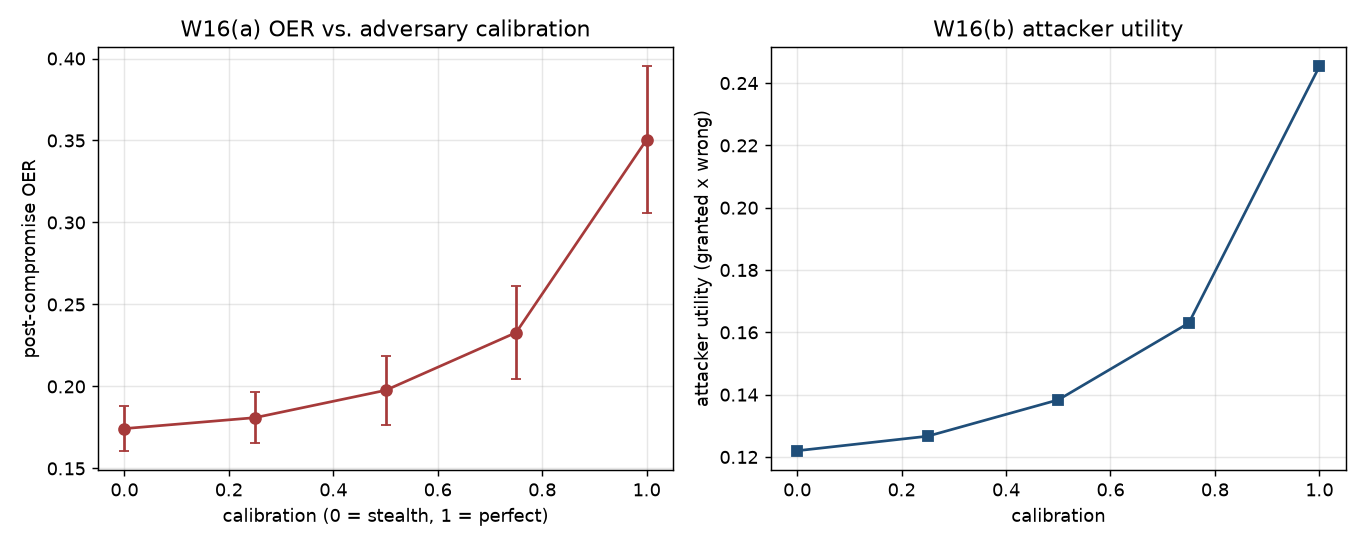
\includegraphics[width=\columnwidth]{figures/w16_adaptive_attacker}}
\caption{E16 (adaptive attacker with calibrated confidence). Behaviour
as the attacker's calibration knob $c$ ranges from $0$ (stealth sleeper
of Assumption~\ref{ass:adversary}: stated confidence $0.95$ regardless
of correctness) to $1$ (stated confidence tracks $\rho{=}0.30$).
\emph{(a)} Post-compromise OER with error bars.  \emph{(b)} Attacker
utility $\mathrm{OER}\cdot(1-\rho)$.  Perfect calibration inflates OER
only by $\times 1.3$ (from $0.17$ to $0.22$) at the cost of a
low-confidence output downstream capabilities are unlikely to act on.}
\Description{Two-panel error-bar plot of OER and attacker utility vs.
the calibration knob c from 0 (stealth) to 1 (perfect), showing modest
increases in both quantities.}
\label{fig:w16}
\end{figure}

% ────────────────────────────────────── H closing remarks
\subsection{Summary}
\label{app:ext_summary}
Taken together, E6--E16 exercise the framework along eleven axes that
prior operational-trust work leaves unmeasured: statistical
significance (E6), colluding adversaries (E7), indirect prompt
injection (E8), per-layer detection attribution (E9), long-horizon
drift (E10), parameter sensitivity (E11), revocation-then-recovery
(E12), Byzantine chains (E13), auditable decisions (E14), calibration
robustness (E15), and adaptive attackers (E16).  Each subsection pairs
an empirical result with a formal statement
(Propositions~\ref{prop:w6}, \ref{prop:w7}, \ref{prop:w9},
\ref{prop:horizon}, \ref{prop:w11}, \ref{prop:w13}, \ref{prop:w14},
\ref{prop:w15}, \ref{prop:w16}; Lemma~\ref{lem:w8};
Corollary~\ref{cor:recovery}) that either reduces the observed
phenomenon to a property of the main-text machinery (typically the
synergy operator, the composite bounds, the Beta-belief fixed point, or
the effective sample horizon) or -- in the case of E7 -- \emph{proves
the negative result} that a naive cross-agent agreement signal cannot
distinguish honest from colluding agents whenever $K\ge 2$.  On every
axis except E7 the observed behaviour is consistent with the theory of
Sections~\ref{sec:model}--\ref{sec:robustness}; E7 identifies
ground-truth-aware agreement statistics, rather than simple majority
counting, as the most important open direction for extending TGCC to
colluding multi-agent scenarios.

\end{document}
